\documentclass[12pt]{amsart}
\usepackage{amsmath,amssymb}
\usepackage{geometry} % see geometry.pdf on how to lay out the page. There's lots.
\geometry{a4paper} % or letter or a5paper or ... etc
% \geometry{landscape} % rotated page geometry

%  POSSIBLY USEFULE PACKAGES
\usepackage{graphicx,caption,subcaption}
\usepackage{tensor}
\usepackage{todonotes}

%  NEW COMMANDS
\newcommand{\pder}[2]{\ensuremath{\frac{ \partial #1}{\partial #2}}}
\newcommand{\ppder}[3]{\ensuremath{\frac{\partial^2 #1}{\partial{align}
      #2 \partial #3} } }
\newcommand{\R}{\ensuremath{\mathbb{R}}}
\renewcommand{\H}{\ensuremath{\mathcal{H}}}
\newcommand{\norm}[1]{\ensuremath{\left\| #1 \right\| }}
\newcommand{\abs}[1]{\ensuremath{ | #1 | }}

%  NEW THEOREM ENVIRONMENTS
\newtheorem{thm}{Theorem}[section]
\newtheorem{prop}[thm]{Proposition}
\newtheorem{cor}[thm]{Corollary}
\newtheorem{lem}[thm]{Lemma}
\newtheorem{defn}[thm]{Definition}
\newtheorem{example}[thm]{Example}

% NEW ENVIRONMENTS

%  MATH OPERATORS
\DeclareMathOperator{\Diff}{Diff}
\DeclareMathOperator{\Dens}{Dens}
\DeclareMathOperator{\SO}{SO}
\DeclareMathOperator{\U}{U}
\DeclareMathOperator{\B}{B}
\DeclareMathOperator{\Fr}{Fr}
\DeclareMathOperator{\Herm}{Herm}
\DeclareMathOperator{\Op}{Op}
\DeclareMathOperator{\Tr}{Tr}
\DeclareMathOperator{\card}{card}
\DeclareMathOperator{\Con}{Con}

%  TITLE, AUTHOR, DATE
\title{Qualitatively accurate spectral schemes for advection}
\author{Henry O. Jacobs \& Ram Vasudevan}
\date{\today}


\begin{document}

\maketitle

\begin{abstract}
  blah blah blah.
\end{abstract}

%%%%%%%%%%%%%%%%%%%%%%%%%%%%%%%%%%%%%%%%%%%%%%%%%%%
\section{Introduction}
\label{sec:intro}

Qualitative accuracy is important because...
Here is an example of a failure.

\subsection{Previous work}
Papers to mention:
\begin{enumerate}
	\item \cite{HenrionKorda2014}
	\item Froyland, Koopman papers
	\item Representation theory stuff \cite{VershilGelfandGraev1975,Ismagilov1975}
	\item Naimark-Gelfand transform 
\end{enumerate}

%%%%%%%%%%%%%%%%%%%%%%%%%%%%%%%%%%%%%%%%%%%%%%%%%%%
\section{Qualitative properties of advection PDEs}
\label{sec:properties}
In this section we define specifically what we mean by ``advection PDEs'' in more precise mathematical terms.
Throughout this paper let $\mathfrak{X}(M)$ denote the space of smooth vector-fields on a compact manifold $M$
and let $X(t) \in \mathfrak{X}(M)$ be a time-dependent vector-field on $M$.
Let $\Phi^{t_{0},t_{1}}_{X}:M\to M$ denote the flow map of $X$ from time $t_{0}$ to $t_{1}$.
Given a bounded real-valued function $f_{0}$, we could consider the time-dependent function $f(x,t) := f_{0} ( (\Phi_{X}^{0,t})^{-1}(x) )$.
The function $f$ represents how $f_{0}$ is pushed and stirred around by the flow of $X$.
For a fixed $x \in M$ we observe, via the chain-rule,
\begin{align}
	 \frac{d}{dt}  f(x;t) &=  \left. \frac{d}{d \epsilon} \right|_{\epsilon=0} ( f(x;t+\epsilon) - f(x,t) ) \\
	 &=  \left. \frac{d}{d \epsilon} \right|_{\epsilon=0} \left( f( (\Phi_{X}^{t,t+\epsilon})^{-1}(x) , t ) - f(x,t) \right) \\
	 &=  \left. \frac{d}{d \epsilon} \right|_{\epsilon=0} \left( f(x,t) + \epsilon \pder{f}{x^{j}} [ (\Phi_{X}^{t,t+\epsilon})^{-1}(x) - x ]^{j} + \mathcal{O}(\epsilon^{2}) - f(x,t) \right) \\
	 &= - X^{j}(x) \pder{f}{x^{j}} = - \pounds_{X}[f_{0}]
\end{align}
where $\pounds_{X}[f]$ denotes the Lie-derivative of $f$.
This calculation yields the time-dependent advection PDE
\begin{align}\label{eq:function pde}
	\pder{f}{t} + X^{j} \pder{f}{x^{j}} = 0.
\end{align}

The same idea works if we consider the advection of a density $\rho_{0}$ by $X$.
In this case, the advected density is given by $\rho (x ; t) =  \det\left[ (D\Phi_{X}^{t,0})^{-1} (x) \right] \rho_{0}( (\Phi_{X}^{0,t})^{-1}(x) )$
and the advection PDE is
\begin{align} \label{eq:density pde}
	\pder{\rho}{t} + \pder{}{x^{j}} \left( \rho X^{j} \right) = 0.
\end{align}

Similarly, a (constant in time) vector-field $Y_{0}$ is advected by $X$ by the formula $Y(x ; t) =  (D\Phi_{X}^{t,0})|_{(\Phi_{X}^{t,0})^{-1}(x)} \cdot Y_{0}( (\Phi_{X}^{t,0})^{-1}(x))$
and satisfies the advection PDE
\begin{align} \label{eq:vector field pde}
	\pder{Y^{i}}{t} + \pder{Y^{i}}{x^{j}} \cdot X^{j} - \pder{X^{i}}{x^{j}} \cdot Y^{j} = 0.
\end{align}

\section{Qualitative properties of advection}
\label{sec:properties}
Advection PDEs preserve a lot of natural structures.
For example if $f(x,t)$ and $g(x,t)$ are solutions to \eqref{eq:function pde}, then the scalar product $f(x,t) g(x,t)$  and the sum $f(x,t) + g(x,t)$ is also a solution to \eqref{eq:function pde}.
This observation can be summarized by the statement \emph{evolution by \eqref{eq:function pde} preserves the ring of functions on $M$}.
In the same vein, if $\rho$ is a density which satisfies \eqref{eq:density pde} and $f$ is a function which satisfies \eqref{eq:function pde}, then the quantity $c = \int_{M} f \cdot \rho$ is constant in time.
This can naturally be extended to the case where $\rho$ is a distribution, and we can summarize this conservation law by saying \emph{advection preserves the duality between functions and distributions on $M$}.

More conservation laws can be found for vector-field advection.
If $Y$ and $Z$ are vector-fields, then there is a natural Lie-bracket structure given by
\begin{align}
	[Y,Z]^{i} \equiv ( \pounds_{Y}[Z] )^{i} := \partial_{j}Z^{i} \, Y^{j} - \partial_{j}Y^{i} \, Z^{j}.
\end{align}
We can observe that if $Y$ and $Z$ satisfy \eqref{eq:vector field pde} then $[Y,Z]$ also satisfies \eqref{eq:vector field pde}.
In summary, advection preserves the Lie algebra of vector fields.

Lastly, the canonical relationships between vector-fields and functions and densities are also preserved.
Given a vector-field $Y$ a function $f$ and a density $\rho$ we may define the Lie derivatives
\begin{align}
	\pounds_{Y}[f] = Y^{j} \partial_{j}f \quad , \quad \pounds_{Y}[\rho] = \pder{}{x^{j}} ( \rho Y^{j} ).
\end{align}
The quantity $\pounds_{Y}[f]$ is itself a function, and $\pounds_{Y}[\rho]$ is a density.
If $f,\rho$ and $Y$ satisfy the advection PDEs \eqref{eq:function pde}, \eqref{eq:density pde}, and \eqref{eq:vector field pde} respectively,
then $\pounds_{Y}[f]$ satisfies \eqref{eq:function pde} and $\pounds_{Y}[\rho]$ satisfies \eqref{eq:density pde}.
In summary, advection preserves the action of vector fields on functions and densities.

In some sense these conservation laws are remarkable, since most PDEs do not conserve all the structures mentioned.
Of course, there is no such thing as magic.
The group of smooth diffeomorphisms of $M$ is in fact identical to the group of ring-automorphisms of $C^{\infty}(M)$.
The formal Lie algebra of the group of Diffeomorphisms is the space of vector-fields $\mathfrak{X}(M)$.
So it is no wonder that advection preserves the ring-structure of functions.
Moreover, the space of distributions is \emph{defined} as the dual space to that of functions, and so the action of a vector-field on distributions is defined
as the dual of the action on functions.
So of course advection preserves the duality between functions and distributions.
Lastly, any Lie group preserves it's own Lie algebra and its own group actions.
So of course advection preserves the Lie bracket of vector fields and the Lie derivatives of functions and densities.
These conservation laws are fundamental properties of advection, and this motivates the definition of qualitative accuracy
which we shall use in this paper:

\begin{center}
    \fbox{
    	\begin{minipage}{0.8\textwidth}
    		A numerical method for an advection is {\bf qualitatively accurate} if it conserves (up to machine precision) the same properties as the exact advection PDE.
    	\end{minipage}
    }
\end{center}

This criterion is separate from numerical accuracy, and can be evaluated independently.
Of course, numerical accuracy takes first priority,
but the goal of this paper will be to go the extra length of constructing a scheme which is numerically
\emph{and qualitatively} accurate.

%%%%%%%%%%%%%%%%%%%%%%%%%%%%%%%%%%%%%%%%%%%%%%%%%%%
\section{The canonical space $L^{2}(M)$}
\label{sec:half densities}
The goal of this paper is to construct a spectral advection scheme which exhibits a large number of invariants.
At the core of many spectral schemes is the use of some Hilbert space upon which everything can be approximated via least squares projections.
Typically this Hilbert space is $L^{2}(M ; \mu)$ where the $L^{2}$-inner product is taken with respect to some non-canonical density or volume form $\mu$ on $M$.
We do not have this luxury.
The properties of advection that we desire to have are strictly properties of $M$ alone, i.e. they are canonical.
Any non-canonical choices we make in constructing our scheme (such as the choice of a volume form) threaten to break these conservation laws by introducing non-canonical artifacts.

In this section we define a geometric version of an $L^{2}$-space which foregoes the choice of a volume form, denoted simply by $L^{2}(M)$.
The ``cost'' we pay for not choosing a volume form is that the elements of $L^{2}(M)$ are not (equivalence classes of) functions because they transform differently under a change of coordinates.

Again, let $M$ be a smooth compact $n$-manifold
and we will let $\Dens(M)$ denote the space of continuous densities,
which we view as anti-symmetric multilinear functions on $\bigoplus^n TM$ \cite[Chapter 16]{Lee2006}.

\begin{defn}\label{def:half density}
	A half-density is a continous complex function $\psi : \bigoplus^n TM \to \mathbb{C}$
	such that $| \psi |^{2} \in \Dens(M)$.
	We denote the space of half densities by $\sqrt{\Dens(M)}$.
\end{defn}

This definition is an equivalent reformulation of the half densities defined in the context of geometric quantization \cite{GuilleminSternberg1970,BatesWeinstein1997}.
In physical terms, $L^{2}(M)$ is precisely the Hilbert space of wave functions on $M$ used in quantum mechanics.
It is unfortunate that physicists call these ``wave-functions''
because elements of $L^{2}(M)$ and $\sqrt{\Dens(M)}$ are \emph{not} functions on $M$.\footnote{However, this sloppy use of names is consistent with others instances such as the fact that the ``Dirac-delta function'' is also not a function.}
One way to see this is to observe how elements of $\sqrt{\Dens(M)}$ transform.
Under a change of coordinates $\Phi$ we observe $\psi$ will map to $\tilde \psi$ where
\begin{align}
	\tilde{\psi}(x)  =  \left| \det \left[ \left. \pder{\Phi^{i}}{x^{j}} \right|_{\Phi^{-1}(x)} \right]_{i,j=1}^{n} \right|^{1/2} \psi( \Phi^{-1}(x) ). \label{eq:transformation law}
\end{align}


As $|\psi|^{2} \in \Dens(M)$ for any $\psi \in \sqrt{\Dens(M)}$ we can integrate $|\psi|^{2}$
and observe that half densities are is naturally equipped with the norm $$\| \psi \|_2 :=  \left( \int_M |\psi|^2 \right)^{1/2}$$ which we call the $2$-norm.

\begin{defn}
	We define $L^{2}(M)$ as the completion of $\sqrt{ \Dens(M)}$ with respect to the $2$-norm.
	The space $L^{2}(M)$ is equipped with a complex inner-product given by
	\begin{align}
		\langle \psi \mid \phi \rangle = \int_{M} \bar \psi \phi
	\end{align}
	through polar decomposition, and so $L^{2}(M)$ is a Hilbert space.
\end{defn}

Lastly, as we know how to transform half-densities, we also know how to advect them.
For a vector-field $X$, the Lie derivative of a half-density is given in local coordinates by
\begin{align}
	\pounds_{X}[\psi] = \frac{1}{2} X^{i} \pder{\psi}{x^{i}} + \frac{1}{2} \pder{}{x^{i}} \left( \psi X^{i} \right). \label{eq:half density pde}
\end{align}
This is an unbounded anti-Hermetian operator on $L^{2}(M)$.
The advection equation can be written as
\begin{align}
	\partial_{t} \psi + \pounds_{X}[\psi] = 0.
\end{align}
By the Stone Von-Neumann theorem \cite{Conway1990}, there is a solution for all time, in spite of the fact that the Lie derivative is an unbounded operator.
Moreover, the solution is given by a unitary action.  For reference later, we restate this remark formally.
\begin{prop} \label{prop:stone}
	The solution to \eqref{eq:half density pde} is of the form $\psi(t) = U(t) \cdot \psi(0)$ where $U(t)$ is
	the unitary operator.
\end{prop}
%\begin{proof}
%	Again, the existence of $U(t)$ as a unitary operator is simply an instance of the Stone Von-Neumann theorem.
%\end{proof}

In fact, $U(t)$ is merely the push-forward operator given in \eqref{eq:transformation law} with ``$\Phi$'' replaced by the flow-map of the dynamics.
We will generally avoid using this explicit expression though, as it can be cumbersome.


\subsection{The relationship with classical $L^{2}$ spaces}
\label{sec:classical_Lebesgue}
For any manifold $M$ (possibly non-orientable) one can assert the existence of a smooth non-negative density $\mu$.
Upon choosing some $\mu$, the $2$-norm of a complex function $f$ with respect to $\mu$ is
\begin{align}
	\| f \|_{\mu,2} =  \left( \int_M |f|^2 \mu \right)^{1/2}.
\end{align}
and $L^2(M ; \mu)$ is the completion of the space of continuous functions with respect to this norm.
The relationship between $L^{2}(M)$ and $L^{2}(M;\mu)$ is that they are identical as topological vector-spaces.
In fact, the isomorphism can be given fairly explicitly.

\begin{prop}
	Choose a non-vanishing density $\mu$.
	Let $\sqrt{\mu}$ be any half-density such that $| \sqrt{\mu} |^{2} = \mu$.
	For any $\psi \in L^2(M)$ there exists a unique $f \in L^2(M ; \mu)$ such that $\psi = f \cdot  \sqrt{\mu}$.
	This yields a continuous isomorphism between $L^2(M)$ and $L^2(M ; \mu)$.
\end{prop}
%\begin{proof}
%	First note that if we view $\mu$ as a positive function on $\bigoplus^n TM$, then we can simply set $\sqrt{\mu}$ to be it's classical square root.
%	It suffices to prove that the dense subspace $\sqrt{\Dens(M)} \subset L^{2}(M)$ can be mapped to a dense subspace of $L^{2}(M;\mu)$ through a map that sends $\| \cdot \|_{2}$ to $\| \cdot \|_{\mu,2}$.
%	
%	Let $\psi \in \sqrt{\Dens(M)}$.  Then $|\psi|^2$ is a continuous density.
%	The Radon-Nikodym derivative of $|\psi|^{2}$ with respect to $\mu$ is a positive valued continuous function $g \in C^0(M)$ defined such that $g \, \mu = |\psi|^2$.
%	Without loss of generality, we may set $g = |f|^{2}$ for some complex function $f$ such that $\psi = f\, \sqrt{\mu}$.
%	The function $f$ is unique with respect to $\psi$ and
%	the map $\psi \in \sqrt{\Dens(M)} \mapsto f \in C^0(M ; \mathbb{C} )$ sends $\| \cdot \|_{2}$ to $\| \cdot \|_{\mu,2}$ by construction.
%	Thus the map is continuous.
%	The inverse of the map is given by $f \in C^{0}(M;\mathbb{C}) \mapsto f \, \sqrt{\mu} \in \sqrt{\Dens(M)}$.
%\end{proof}

At this point the reader might ask ``If both space are the same, then why don't we use the one that is more familiar?  i.e. the space $L^{2}(M;\mu)$''.
The answer is that these space are really not the same in all aspects.
One difference that we've already discussed is that they transform differently.
Elements of $L^{2}(M)$ transform according to \eqref{eq:transformation law} while elements of $L^{2}(M;\mu)$ transform like functions.
Additionally, a more useful difference for us is that $L^{2}(M)$ is \emph{not} contained within $L^{1}(M)$ and $L^{\infty}(M)$ is not contained in $L^{2}(M)$
because each of these spaces consists of objects with different transformation properties.
This separation between $L^{2}(M)$ and $L^{1}(M)$ \emph{forces} us to think of these objects as distinct.
For example an operator on $L^{2}(M)$ can not generally be applied to $L^{1}(M)$ in the same way.
Later we will find this is a good thing, because it allows us to have an operator act on $L^{1}(M)$ differently than how it acts on $L^{2}(M)$
without leading to contradiction.
Such safety mechanisms are analogous to the use of private/public functions in object oriented programming, which place constraints on a computer program in order to banish certain bugs from arising.

\subsection{Sobolev spaces}
\label{sec:Sobolev spaces}
For each $X \in \mathfrak{X}(M)$ the operator $\pounds_{X}$ on $L^{2}(M)$ is unbounded.
In the parlance of functional analysis, the domain of $\pounds_{X}$ is
\begin{align}
	\operatorname{dom}( \pounds_{X} ) := \{ \psi \in L^{2}(M) \mid  \| \pounds_{X}[\psi] \|_{L^{2}} < \infty \}.
\end{align}
One can then show that $\operatorname{dom}( \pounds_{X} )$ is a closed subspace of $L^{2}(M)$ and then define
a \emph{canonical} Sobolev space
\begin{align}
	H^{1}(M) := \bigcap_{X \in \mathfrak{X}(M)} \operatorname{dom}( \pounds_{X} ).
\end{align}
Where we view $\pounds_{X}$ as an unbounded operator on $L^{2}(M)$.
More generally, we can construct $H^{k}(M)$ by composing multiple Lie derivative operators,
and we can even consider fraction degrees of regularity as well.
%As $\pounds_{X}$ is anti-Hermetian we can invoke the spectral theorem of functional analysis
%and consider the operator
%\begin{align}
%	(\pounds_{X})^{s} [ \psi] = \sum_{\lambda \in \sigma( \pounds_{X}) } \lambda^{s} \langle e_{\lambda} \mid \psi \rangle e_{\lambda}
%\end{align}
%where $\{ e_{\lambda} \mid \lambda \in \sigma( \pounds_{X}) \}$ denotes the set of eigenvectors of $\pounds_{X}$. 
%This fractional power of $\pounds_{X}$ allows us to consider Sobolev spaces of fractional orders as well.

  However, while the canonicalism of $L^{2}(M)$ will be quite useful to us,
  \emph{canonical} (metric-free) Sobolev spaces will not be.
  We will find that our algorithms only converge on spaces of sufficient regularity,
  but in order to perform our error-analysis we will need to choose a non-canonical norm.
  
To begin the process of choosing a norm for $H^{s}(M)$, equip $M$ with a Riemannian metric $g:TM \oplus TM \to \mathbb{R}$.
The metric induces a positive density $\mu_g$,
known as the \emph{metric density}. 
The Riemmanian density induces the $L^2$ inner-product on $C^\infty(M)$ via
\begin{align}
	\langle f_1 , f_1 \rangle_{g} = \int \overline{f_1} \cdot f_2 \mu_g
\end{align}
and $L^{2}(M;\mu_{g})$ is the completion of the inner-product space $( C^{\infty}(M) , \langle \cdot , \cdot \rangle_{g})$ under 
the inner-product norm.
The metric also induces an elliptic operator, known as the Laplace-Beltrami operator $\Delta: C^{\infty}(M) \to C^{\infty}(M)$, which is is positive-semidefinite
with respect to $\langle \cdot , \cdot \rangle_{g}$.
If $M$ is compact, then $L^2(M ; \mu_g) \cong L^2(M)$ is a separable Hilbert space
and the Helmholtz operator, $1 + \Delta$, is then a positive definite operator
with a discrete spectrum.
For any $s \geq 0$ we may define the Sobolev norm
\begin{align}
	\| f \|_{s,2} =  \left( \langle f , (1+\Delta)^s \cdot f \rangle_{g} \right)^{1/2}
\end{align}
and $H^s(M ; g)$ is then the function space obtained by completion with respect to this norm, and modulo discrepancies of measure zero.
Note that $H^0(M;g) = L^2(M;\mu_g)$.

The following proposition will be of use later when we need to prove a notion of convergence
via sequences of finite rank operators.

\begin{prop} \label{prop:compact_embedding}
	Let $(M,g)$ be a compact Riemmanian manifold.  If $s > t \geq 0$ then $H^s(M;g)$ is compactly embedded within $H^t(M,g)$.
\end{prop}
\begin{proof}
	As $M$ is compact we know that the spectrum of $\Delta$ is discrete and $L^{2}(M)$ is separable.
	Let $e_0, e_1,\dots$ be the Hilbert basis for $L^2(M;\mu_g)$ which diagonalizes $\Delta$
	in the sense that $\Delta e_i = \lambda_i e_i$ for a sequence $0 = \lambda_0 \leq \lambda_1 \leq \lambda_2 \leq \cdots$.
	The operator $(1+\Delta)^s$ is given by
	\begin{align}
		(1+\Delta)^s \cdot f =  \sum_{i} e_i (1+\lambda_i)^s \langle e_i , f \rangle_g,
	\end{align}
	and so $\{ (1+ \lambda_i)^{-s} e_i \}_{i=1}^{\infty}$ is a Hilbert basis for $H^s(M;g)$.
	
	Let us call $e_i^{(s)} = (1+ \lambda_i)^{-s} e_i$.
	The embedding of $H^s(M;g)$ into $H^t(M,g)$
	is then given in terms of the respective basis elements by $e_i^{(s)} \mapsto (1+\lambda_i)^{-(s-t)}e_i^{(t)}$.
	As $s > t$ and $\lambda_i \to +\infty$, we see that 
	this embedding is a compact operator \cite[see Proposition 4.6]{Conway1990}.
\end{proof}

In the sequel we shall say that $\psi \in L^2(M)$ is of class $H^s$ if $\psi = f \sqrt{\mu_g}$, and $f \in H^s(M,g)$.
That $\psi$ is of class $H^{s}$ is topological statement, and not metric dependent.
However, the norm $\| \psi \|_{2,s} = \| f \|_{2,s}$ is metric dependent.

\section{A spectral discretization}
The goal of this section will be to produce a spectral scheme for the advection equations \eqref{eq:function pde}, \eqref{eq:density pde}, and \eqref{eq:vector field pde}
using the space $L^{2}(M)$.
In order to realize this goal we must relate functions, densities, and vector-fields to $L^{2}(M)$ in a way that can be spectrally discretized without breaking any canonical structures.

To begin, let us consider the space of continuous real-valued functions $C(M)$.
For each $f \in C(M)$ there is a unique bounded Hermetian operator, $\hat{f} : L^{2}(M) \to L^{2}(M)$ given by scalar multiplication.
That is to say $(\hat{f} \cdot \psi) (x) = f(x) \psi(x)$.
We see that the hat-map, $f \mapsto \hat{f}$, preserves the ring structure because $\widehat{f \cdot g + h} = \hat{f} \cdot \hat{g} + \hat{h}$.

Similarly, (and in the opposite direction) for any trace class operator $\hat{\rho}$ there is a unique distribution $\rho \in C(M)'$ such that 
\begin{align}
	 \int f \, \rho = \Tr ( \hat{f}^{\dagger} \cdot \hat{\rho} )
\end{align}
for any $f \in C(M)$.
By construction, the surjection $\hat{\rho} \mapsto \rho$ and the injection $f \mapsto \hat{f}$ preserve the duality between functions and distributions.

Finally, for any vector field $X$ there is a unique (unbounded) anti-symmetric operator $\pi(X)$ on $L^{2}(M)$
given in coordinates by
\begin{align}
	\pi(X) \cdot \psi = \frac{1}{2} X^{j} \pder{\psi}{x^{j}} + \frac{1}{2} \pder{}{x^{j}} ( \psi \, X^{j} ). \label{eq:representation}
\end{align}
After some minor computations (see Appendix \ref{app:Lie} \todo{need to write an appendix} ) we see that $\pi$ is a Lie algebra morphism which sends
the Jacobi-Lie bracket to (minus) the commutator bracket.  That is to say, $\pi$ is linear and $\pi([X,Y]) = - [ \pi(X) , \pi(Y)]$.

\begin{example}
Let us describe what this means when $M$ is a torus.
In standard coordinates $\theta = (\theta^{1},\dots,\theta^{d})$ we may write $X = X^{i}(\theta) \frac{\partial}{\partial \theta^{i}}$ for some functions $X^{1}(\theta),\dots,X^{d}(\theta)$.
In a Fourier basis $\{ \frac{1}{\sqrt{2\pi}} e^{ i \langle k , \theta \rangle}   \mid k \in \mathbb{Z}^{d} \}$ 
a half density, $\psi$ is given by it's Fourier series $\mathcal{F}[\psi]$.
Upon noting that $\mathcal{F}[ f \cdot \psi] = \mathcal{F}[f] * \mathcal{F}[\psi]$
we find $\hat{f} = \mathcal{F}[f] * $, i.e. $\hat{f}$ is the convolution operator associated to the Fourier transform of $f$.
We observe that $\pi \left( \pder{}{\theta^{j}} \right) \cdot e^{i \langle k , \theta \rangle}  = i k^{j} e^{i \langle k,\theta\rangle}$.
That is to say, $\pi \left( \pder{}{\theta^{j}} \right)$ simply multiplies the $k$th mode by $k^{j}$.
This is the sparsest representation of this operator one can ever expect to obtain.
We then see that $\pi(X) \cdot \psi = \mathcal{F}[X^{j}] *  [ \pi \left( \pder{}{\theta^{j}} \right) \cdot \psi ]$.
If $X$ is smooth, than $\mathcal{F}(X^{j})$ is well approximated by a sparse operator by truncation.
As a result, we have a sparse spectral approximation of $\pi(X)$ when we use truncation.

Finally, given a sufficiently regular\footnote{e.g. $W^{1+\epsilon,1}$ for $\epsilon >0$ will do.} density, $\rho$,  we could 
split $\rho$ into non-negative and non-positive components as $\rho = \rho^{+} - \rho^{-}$
so that $\psi = \sqrt{\rho^{+}} + i \sqrt{\rho^{-}}$ is a square root of $\rho$.
Then $\hat{\rho}$ is represented in the Fourier domain by $\mathcal{F}(\psi) \otimes \mathcal{F}(\psi)^{\dagger}$.
\end{example}

We can now convert the evolution PDEs \eqref{eq:function pde}, \eqref{eq:density pde}, and \eqref{eq:vector field pde}
into ODE's of operators on $L^{2}(M)$.

\begin{thm} \label{thm:quantize}
	Let $X(t) \in \mathfrak{X}(M)$ be a time-dependent vector-field.
	Then $f$, $\rho$, and $Y$ satisfy \eqref{eq:function pde},\eqref{eq:density pde}, and \eqref{eq:vector field pde} respectively
	if and only if $\hat{f}$, $\hat{\rho}$, and $\pi(Y)$ satisfy the operator ODEs
	\begin{align}
		&\frac{d \hat{f} }{dt} + [ \hat{f} , \pi(X) ] = 0 \label{eq:quantum observable ode} \\
		&\frac{d \hat{\rho} }{dt} + [ \hat{\rho} , \pi(X) ] = 0 \label{eq:quantum density ode} \\
		&\frac{d \pi(Y) }{dt} + [ \pi(Y), \pi(X) ] = 0 \label{eq:quantum vf ode}
	\end{align}
	respectively.
	Moreover, if $\psi \in L^{2}(M)$ is such that $\psi^{2} = \rho$ and $\psi$ satisfies \eqref{eq:half density pde}, then $\rho$ satisfies \eqref{eq:density pde}.
\end{thm}

\begin{proof}
	Let $f$ satisfy \eqref{eq:function pde}.
	For an arbitrary $\psi \in L^{2}(M)$ we observe that $[ \hat{f} , \pi(X)] \cdot \psi$ is given in coordinates by
	\begin{align}
		[ \hat{f} , \pi(X) ] \cdot \psi = f \left( \frac{1}{2} X^{j} \pder{\psi}{x^{j}} + \frac{1}{2} \pder{}{x^{j}} ( \psi \, X^{j} ) \right)
			- \frac{1}{2} X^{j} \pder{}{x^{j}}( f \psi)  + \frac{1}{2} \pder{}{x^{j}} (f \psi \, X^{j} )
	\end{align}
	where we have used \eqref{eq:representation}.  Application of the product rule to all these terms then yields
	a number of cancellations and we find
	\begin{align}
		[ \hat{f} , \pi(X) ] \cdot \psi = - X^{j} \pder{f}{x^{j}} \psi = (\partial_{t} f )\psi = \frac{d \hat{f} }{dt} \cdot \psi.
	\end{align}
	As $\psi$ is arbitrary we have managed to show that $\hat{f}$ satisfies \eqref{eq:quantum observable ode}.
	Each line of reasoning is reversible, and so we have proven the converse as well.
	
	In order to handle densities note that $\langle f , \rho \rangle = \int_{M} f\rho$ is constant in time when $f$
	and $\rho$ satisfy \eqref{eq:function pde} and \eqref{eq:density pde} respectively.
	By the definition of $\hat{\rho}$ we observe $\Tr( \hat{f}^{\dagger} \hat{\rho}) = \langle f , \rho \rangle$.
	Thus we find
	\begin{align}
		0 = \frac{d}{dt} \left( \Tr( \hat{f}^{\dagger} \rho ) \right) = \Tr \left( \frac{d \hat{f}^{\dagger}}{dt} \hat{\rho} + \hat{f}^{\dagger} \frac{d \hat{\rho}}{dt} \right).
	\end{align}
	As was just shown, $\frac{d}{dt} \hat{f} =  - [\hat{f} , \pi(X) ]$ so we observe
	\begin{align}
		0 = \Tr( - [\hat{f} , \pi(X) ]^{\dagger} \hat{\rho} + \hat{f}^{\dagger} \hat{\rho} ) = \Tr( - \pi(X)^{\dagger} \hat{f}^{\dagger} \hat{\rho} + \hat{f}^{\dagger} \pi(X)^{\dagger} \hat{\rho} + \hat{f}^{\dagger} \frac{d\hat{\rho}}{dt} ).
	\end{align}
	Upon noting that $\pi(X)^{\dagger} = - \pi(X)$ and use of identity $\Tr( a b c) = \Tr( bc a)$ we obtain
	\begin{align}
		0 = \Tr \left( \hat{f}^{\dagger}( [\hat{\rho} , \pi(X) ] + \frac{d \hat{\rho}}{dt} ) \right).
	\end{align}
	As $\hat{f}$ was chosen arbitrarily, the desired result follows.
	Again, this line of reasoning is reversible.
	
	Thirdly, if $Y$ satisfies \eqref{eq:vector field pde}, then we observe 
	\begin{align}
		\frac{d}{dt} \pi(Y) = \pi ( \partial_{t} Y ) = \pi( - [X,Y] ) = [\pi(X) , \pi(Y) ].
	\end{align}
	where we have used the fact that $\pi$ is bracket preserving.
	
	Lastly, if $\psi$ satisfies \eqref{eq:half density pde} and $\rho = \psi^{2}$ then we see
	\begin{align}
		\partial_{t} \rho &= \partial_{t} ( \psi^{2}) = 2 (\partial_{t} \psi ) \, \psi \\
		&= 2 \left( - \frac{1}{2} \partial_{i} (\psi X^{i}) - \frac{1}{2} X^{i} \partial_{i} \psi \right) \psi \\
		&= \left( - X^{i} \partial_{i} \psi - \psi \partial_{i} X^{i}  \right) \psi \\
		&= - 2 \psi (\partial_{i} \psi) X^{i} - (\partial_{i}X^{i}) \psi^{2}\\
		&= - \partial_{i}(\rho) X^{i} - (\partial_{i}X^{i}) \rho = - \partial_{i} ( \rho X^{i}).
	\end{align}
\end{proof}


The benefit of representing our pde's in the form \eqref{eq:quantum observable ode},\eqref{eq:quantum density ode}, and \eqref{eq:quantum vf ode}
is that we may construct discretization schemes for these equations using least squares projections.
In particular choose a metric, $g$, and let $\{ f_{0}, f_{1},\dots \}$ denote  eigen-functions of the Laplace operator.
Then $\{ f_{0} \sqrt{\mu_{g}} , f_{1} \sqrt{\mu_{g}} , \dots \}$ forms a smooth Hilbert basis for $L^{2}(M)$ where $\mu_{g}$ denotes the Riemmannian density.
Let $V_{n}$ denote the span of the first $n+1$ elements.
Let $\pi_{n}:L^{2}(M) \to V_{n}$ denote the orthogonal projection. 
Given these choices we obtain the following numerical scheme for \eqref{eq:function pde}

\begin{center}
\fbox{ \label{function scheme}
	\begin{minipage}{0.8\textwidth}
		{\bf Algorithm 1:} An algorithm for functions.\\
		{\bf Problem:} Given an initial condition $f(0) \in C(M)$ solve \eqref{eq:function pde} on the time interval $[0,T]$.\\
		{\bf Numerical solution:}
		\begin{enumerate}
			\item Let $\hat{f}_{n}(0) := \pi_{n} \cdot \hat{f}(0) |_{V_{n}}$ and $X_{n} := \pi_{n} \cdot \pi(X) |_{V_{n}}$.
			\item Solve the finite dimensional ode $\frac{d}{dt} \hat{f}_{n} + [ \hat{f}_{n} , X_{n} ] = 0$ with initial condition $\hat{f}_{n}(0)$ on the interval $[0,T]$.
		\end{enumerate}
	\end{minipage}
}
\end{center}

This algorithm is more provided out of theoretical interest, than of a practical suggestion.
The size of the matrix $\hat{f}_{n}$ is $n^{2d}$, and even if it is sparse initially it will become dense when $t$ increases.
This is prohibitively expensive at $d = 3$.
On the torus, a more practical approach which holds much of the numerical benefits would be to approximate $\hat{f}_{n}$ psuedo-spectrally,
by evaluating $f$ on grid points.
The resulting method is really the method of characteristics in disguise (i.e. a particle method).

\begin{center}
\fbox{ \label{psuedo spectral scheme}
	\begin{minipage}{0.8\textwidth}
		{\bf Algorithm 1b:} A psuedo-spectral algorithm for Toric functions.\\
		{\bf Problem:} Given an initial condition $f(0) \in C( \mathbb{T}^{n} )$ solve \eqref{eq:function pde} on the time interval $[0,T]$.\\
		{\bf Numerical solution:}
		\begin{enumerate}
			\item Initialize a regular grid, $\Omega_{n}$, of size $n = r^{d}$.
			\item Solve the ode $\dot{y}_{i}(t) = X(y_{i})$ with the initial condition $y_{i}(0) = x_{i}$ for each $x_{i} \in \Omega_{n}$.  
			\item Set $\hat{f}_{n}$ to be the truncated convolution operator associated 
				to the Fourier series $\mathcal{DFT}[ f_{0}(y_{1}(t)) , \dots, f_{0}(y_{n}(t) ) ]$,
				where $\mathcal{DFT}$ denotes the discrete Fourier transform.
		\end{enumerate}
	\end{minipage}
}
\end{center}

The use of the discrete Fourier transform introduces errors which disrupt the conservation laws we seek to keep.
However, these newly incurred errors are dominated by other discretization errors, which we still analyze shortly.
While our main concern in this paper is with the properties of algorithm 1, we merely mention algorithm 1b as a practical alternative
that still retains much of the benefits.

%The final step might require explanation.
%It will be shown that as $n$ increases $\hat{f}_{n}(t)$ converges to the solution, $\hat{f}$, of \eqref{eq:quantum observable ode} with respect to the operator norm.
%By theorem \eqref{thm:quantize} we know that the solution of \eqref{eq:quantum observable ode} is related to the solution of \eqref{eq:function pde}
%through the map $f \mapsto \hat{f}$.
%If one desires to get a function rather than an operator we must find a left inverse of the hat-map because $\hat{f}_{n}$ will typically fall outside the range of the hat-map.
%This is what is accomplished in step (4) where an optimization problem yields a local left inverse function.
%As the operator norm is identical to the supremum norm it is possible to show that $f_{n}(t)$ converges to $f$ in the sup-norm.

To solve the Louiville equation, \eqref{eq:density pde}, we could implement the following
\begin{center}
\fbox{
	\begin{minipage}{0.8\textwidth}
		{\bf Algorithm 2:} An algorithm for densities.\\
		{\bf Problem:} Given $\rho_{0} \in \Dens(M)$ solve \eqref{eq:density pde} on the time interval $[0,T]$.\\
		{\bf Numerical solution:}
		\begin{enumerate}
			\item Split $\rho_{0} = \rho_{0}^{(+)} - \rho_{0}^{(-)}$ for positive densities, $\rho_{0}^{(+)},\rho_{0}^{(-)}$.
			\item Let $\psi_{0} = \sqrt{ \rho_{0}^{(+)}} + i \sqrt{\rho_{0}^{(-)}}$.
			\item Solve \eqref{eq:half density pde} numerically with initial conditions $\psi_{0}$. (see algorithm 3)
			\item Set $\rho(t) = \psi(t)^{2}$. 
		\end{enumerate}
	\end{minipage}
}
\end{center}

Step (3) of the above algorithm involves solving \eqref{eq:half density pde} numerically.
Here we propose the most naive spectral algorithm
\begin{center}
\fbox{
	\begin{minipage}{0.8\textwidth}
		{\bf Algorithm 3:} An algorithm for half densities. \\
		{\bf Problem:} Given and initial condition $\psi(0) \in H^{s}(M)$ solve \eqref{eq:half density pde} on the time interval $[0,T]$.\\
		{\bf Numerical solution:}
		\begin{enumerate}
			\item set $[X]_{n} = \pi_{n} \cdot \pi(X) |_{V_{n}}$.
			\item We observe that $[X]_{n}$ is a linear automorphism on a finite dimensional subspace.
			Thus we can solve the ODE $\frac{d\psi_{n}}{dt} = [X]_{n} \cdot \psi_{n}$ with the initial condition $\psi_{n}(0) = \pi_{n}(\psi(0))$
			using a standard ODE integrator.\footnote{We use the implementation of VODE \cite{VODE} within SciPy \cite{Scipy} in this paper.}
		\end{enumerate}
	\end{minipage}
}
\end{center}

While half-densities and algorithm 3 may be of little interest in most problems,
we will find that being able to solve \eqref{eq:half density pde} accurately will be crucial in determining the accuracy of algorithms 1 and 2 (i.e. solving \eqref{eq:function pde} and \eqref{eq:density pde}).

\section{Error analysis}

This article concerns a collection of numerical schemes (one for half-densities, one for densities, one for functions, etc) and a priori one might think we will need to perform a lot of error analysis.
However, the saving grace of our schemes is that they are all connected.  We will find that error bounds for our schemes can be derived as functions of an error bound
for our numerical solution to \eqref{eq:half density pde}.  Therefore we will prioritize deriving a useful error bound for a solution
of \eqref{eq:half density pde}.

Let us begin by observing how well half densities in $V_{n}$ can approximate arbitrary members of $H^{s}(M)$.

\begin{prop} \label{prop:approximation}
	Let $\psi \in H^{\bar{s}}(M)$ for $\bar{s} > s \geq 0$.
	Then
	\begin{align}
		\| \psi - \pi_{n}(\psi) \|_{H^{s}} <  \frac{d \, C_{\bar{s},s} }{ \bar{s}-s} \| \psi \|_{H^{\bar{s}}} \, n^{-2(\bar{s}-s)/d}
	\end{align}
	for some constant $C_{\bar{s},s}$ and $d = \dim(M)$.
\end{prop}
\begin{proof}
	The Fourier decomposition of $\psi$ satisfies
	\begin{align}
		\| \psi \|^{2}_{H^{\bar{s} }} = \sum_{k=0}^{\infty} \hat{\psi}_{k}^{2} (1+\lambda_{k})^{\bar{s}} < \infty
	\end{align}
	Weyl's asymptotic formula tells us that $\lambda_{k} \sim k^{2/d}$.
	Substitution of this asymptotic result into the above inline equation for large $k$ tells us that $\hat{\psi}_{k}^{2}$ is asymptotically dominated by  $C k^{-1- 2\bar{s}/d}$
	for some constant $C$.
	Let $n$ be such that this dominance occurs for all $k>n$.  Then we find
	\begin{align}
		\| \psi - \pi_{n}(\psi) \|_{H^{s}} = \sum_{k>n} (1+\lambda_{k})^{s} \hat{\psi}_{k}^{2} \leq C \sum_{k>n} (1+\lambda_{k})^{s} k^{-1- 2\bar{s}/d}
	\end{align}
	and by another application of the Weyl formula
	\begin{align}
		\| \psi - \pi_{n}(\psi) \|_{H^{s}} \leq \tilde{C} \sum_{k>n} \frac{1}{k^{1+2(\bar{s}-s)/d}} \leq C_{s,\bar{s}}  \frac{d }{ \bar{s}-s} n^{-2(\bar{s}-s)/d}.
	\end{align}
	Where the last inequality is derived by bounding the above infinite sum with an integral.
\end{proof}

We should note that this error bound illustrates that we have a spectral convergence rate on smooth data.
This rapid convergence for smooth data will trickle down to algorithms 1 and 2 as well.
Now that we have derive an error bound for the approximation error of $V_{n}$ with respect to $H^{s}(M)$ we can 
derive an error bound for the numerical solutions derived in algorithm 3.

\begin{thm} \label{thm:half density convergence}
	Let $\psi_{0} \in H^{\bar{s}}(M)$ for $\bar{s} > s > 1$.
	Let $\psi(t)$ be the exact solution to \eqref{eq:half density pde} with initial condition $\psi_{0}$ and let
	and $\psi_{n}(t)$ be the numerical solutions on the interval $[0,T]$ for $T < \infty$ with initial condition $\psi_{n}(0) = \pi_{n}(\psi_{0})$
	computed using algorithm 3.
	Then the error $E_{n}(t) := \| \psi(t) - \psi_{n}(t) \|_{H^{s}}$ satisfies the bound
	\begin{align}
		E_{n}(t) \leq \| \psi_{0} \|_{H^{\bar{s}}} \, K \left( n^{-2(s-1)} t+  \frac{d}{\bar{s}-s} n^{-2(\bar{s}-s)/d} \right) e^{C t}
	\end{align}
	for all $t \in [0,T]$, where $K$ and $C$ are positive constants with respect to $n$,$s$, and $\bar{s}$.
	In particular for $s = (\bar{s}+1)/2$ we get
	\begin{align}
			E_{n}(t) \leq \| \psi_{0} \|_{H^{\bar{s}}} \, K \left( n^{1-\bar{s}} t+  \frac{d}{\bar{s}-1} n^{(1-\bar{s})/d} \right) e^{C t}.
	\end{align}
\end{thm}



\begin{proof}
	Note that $\frac{dE_{n}}{dt} = \frac{1}{2E_{n}} \langle  \psi - \tilde{\psi} \mid \frac{d}{dt} ( \psi -\tilde{\psi} )\rangle_{H^{s}}$.
	By the Cauchy-Schwarz inequality we see that
	\begin{align}
		\frac{dE_{n}}{dt} &\leq  \frac{1}{2} \| X[\psi] - \pi_{n}(X[\psi_{n}]) \|_{H^{s}} = \| X[\psi] - \pi_{n}( X[\psi- (\psi-\psi_{n})]) \|_{H^{s}} \\
	\intertext{By the triangle inequality we may split this sum and use the definition of the operator norm to find}
		&\leq \| (1-\pi_{n})|_{H^{s-1}} \|_{op} \, \|X|_{H^{s}} \|_{op} \, \| \psi \|_{H^{s}} + \| \pi_{n} \| \, \|X|_{H^{s}} \| \, E_{n} \\
	\end{align}
	We know $\psi(t) = \Phi^{t}_{*}\psi_{0}$ where $\Phi^{t}$ is the flow of $X$.
	As $\Phi$ is as smooth as $X$ we can see that $\| \psi(t) \|_{H^{s}}$ is bounded by a scalar multiple of $\| \psi_{0} \|_{H^{s}}$.
	Thus we may write the above bound in the form
	\begin{align}
		\frac{dE_{n}}{dt} \leq K' \, \| (1- \pi_{n})|_{H^{s-1}} \| \, \| \psi_{0}\|_{H^{s}}+ C E_{n}
	\end{align}
	for constants $C$ and $K'$.
	We can explicitly compute $\| (1-\pi_{n})|_{H^{s-1}} \|_{op} = (1+\lambda_{n+1})^{-(s-1)}$ where $\lambda_{k}$ denotes the $k$th eigenvalue of the Laplace operator.
	By Weyl's asymptotic formula \cite[Theorem B.2]{Chavel1984} we
	can derive that $\lambda_{n}$ asymptotically behaves like $n^{2/d}$ where $d = \dim(M)$.
	Therefore by a perturbed version of Gronwall's inequality (see Lemma \ref{lem:Gronwall} on page \pageref{lem:Gronwall}) with $\epsilon = C_{1,T} n^{-2(s-1) / d} \, \| \psi_{0}\|_{H^{s}}$
	we find
	\begin{align}
		E(t) \leq ( K' n^{-2(s-1) / d} \| \psi_{0} \|_{H^{s}} t+  E(0) ) e^{C t}.
	\end{align}
	That $E_{n}(0)$ behaves as $K'' \| \psi_{0} \|_{H^{\bar{s}}} n^{-2(\bar{s}-s)/d}$ is merely a re-statement of Proposition \ref{prop:approximation}.
	We then set $K = \max(K', K'')$.
\end{proof}

Having derived an error bound for algorithm 3, we can also derive an error bound for algorithm 2.

\begin{thm} \label{thm:density convergence}
	Let $\rho(0)$ be a distribution in $W^{\bar{s},1}(M)$ for $\bar{s} > s >1$.
	Let $\rho(t)$ be the solution of \eqref{eq:density pde} on the time interval $[0,T]$.
	Let $\rho_{n}(t)$ be the numerical solution derived via algorithm 2 on the time interval $[0,T]$.
	Then we find
	\begin{align}
		\| \rho(t) - \rho_{n}(t) \|_{L^{1}} \leq \| \rho(0) \|_{W^{\bar{s},1}} \, \bar{K} \left( n^{-2(s-1)} t+  \frac{d}{\bar{s}-s} n^{-2(\bar{s}-s)/d} \right) e^{C t}
	\end{align}
	for all $t \in [0,T]$, $\bar{K}$ is constant with respect to $n$ and $C$ is the same constant as in Theorem \ref{thm:half density convergence}.
\end{thm}

\begin{proof}
	Without loss of generality, we can assume that $\rho$ is non-negative (otherwise split it into it's non-negative and non-positive components).
	Let $\psi \in L^{2}(M)$ be such that $\rho =  \psi ^{2}$, as described in algorithm 2.
	It follows that $\psi \in H^{s}(M)$ and we compute
	\begin{align}
		\| \rho(t) - \rho_{n}(t) \|_{L^{1}} = \int_{M} | \rho(t) - \rho_{n}(t)| = \int_{M} | \psi^{2} - \psi_{n}^{2} |
	\end{align}
	If we let $\phi_{n} = \psi - \psi_{n}$ then we can re-write the above as
	\begin{align}
		\| \rho(t) - \rho_{n}(t) \|_{L^{1}}  &= \int_{M} | \psi^{2} - (\psi - \phi_{n})^{2} | = \int_{M} | 2 \psi \phi_{n} - \phi_{n}^{2} | \\
			&\leq 2 \| \psi \|_{L^{2}} \| \phi_{n}\|_{L^{2}} + \| \phi_{n} \|_{L^{2}}^{2} = 2 \| \rho \|_{L^{1}}^{1/2} \cdot \| \phi_{n} \|_{L^{2}} + \| \phi_{n} \|_{L^{2}}^{2}
	\end{align}
	By Theorem \ref{thm:half density convergence} provides a bound for $\| \phi_{n} \|$.
	Substitution of this bound into the above inequality yields the theorem.
\end{proof}

Finally, we show that algorithm 1 converges to a solution of \eqref{eq:quantum observable ode}, which is morally equivalent to a solution
of \eqref{eq:function pde} courtesy of Theorem \ref{thm:quantize}.

\begin{prop} \label{prop:function approximation}
	Let $f \in C^{k}(M)$ and let $\hat{f}_{n} = \pi_{n} \circ \hat{f} \circ \pi_{n}$.  Then
	\begin{align}
		\| ( \hat{f} - \hat{f}_{n} )|_{H^{s}} \|_{op} \leq D \frac{d}{s} n^{-2s/d} \| \hat{f} \|_{op}
	\end{align}
	where $d= \dim(M)$, $s > k \geq 1$, and $D$ is constant.
\end{prop}
\begin{proof}
	Let $\pi_{n}^{\perp} = 1 - \pi_{n}$.  By Proposition \ref{prop:approximation} we know that
	\begin{align}
		\| \pi_{n}^{\perp}(\psi) \|_{L^{2}} \leq \frac{d}{s} n^{-2s/d} \| \psi \|_{H^{s}} \label{eq:hot inequality}
	\end{align}
	for $s>0$.  We now use this to compute the desired bound.  We find
	\begin{align}
		\| (\hat{f} - \hat{f}_{n})|_{H^{s}} \|_{op} &= \sup_{\| \psi \|_{H^{s}}=1} \langle \psi \mid \hat{f} - \hat{f}_{n} \mid \psi \rangle \\
			&= \sup_{\| \psi \|_{H^{s}}=1} \left( \langle \psi \mid \hat{f}  \mid \psi \rangle - \langle \psi - \pi_{n}^{\perp}(\psi) \mid \hat{f} \mid \psi - \pi_{n}^{\perp}(\psi) \rangle \right) \\
			&= \sup_{\| \psi \|_{H^{s}}=1} \left( 2 \Re \langle \pi_{n}^{\perp}(\psi) \mid \hat{f} \mid \psi \rangle - \langle \pi_{n}^{\perp}(\psi) \mid \hat{f} \mid \pi_{n}^{\perp}(\psi) \rangle \right) \\
			&\leq \sup_{\| \psi \|_{H^{s}}=1}  ( \| \pi_{n}^{\perp}(\psi) \|_{L^{2}}- \| \pi_{n}^{\perp}(\psi) \|_{L^{2}}^{2} ) \| \hat{f} \|_{op} \\
	\end{align}
	By \eqref{eq:hot inequality} the result follows.
\end{proof}

\begin{thm} \label{thm:function convergence}
	Let $f(t) \in C^{k}(M)$ be a solution to \eqref{eq:function pde} so that $\hat{f}(t)$ is a solution to \eqref{eq:quantum observable ode}.
	Let $\hat{f}_{n}$ denote the numerical solution obtained through the numerical scheme described on page \pageref{function scheme}.
	Then
	\begin{align}
		\| ( \hat{f} - \hat{f}_{n})|_{H^{s}} \|_{op} \leq D \frac{d}{s} n^{-2s/d} \| \hat{f} \|_{op}+  K \| \hat{f}_{n} \|_{op} \left( n^{1-s} + \frac{2d}{s -1} n^{(1-s)/d} \right) e^{Ct}
	\end{align}
	for the same constants $D$ as in Proposition \ref{prop:function approximation} and the same constants $C,K$ as in \ref{thm:half density convergence}.
\end{thm}

\begin{proof}
	We find
	\begin{align}
		\| ( \hat{f}(t) - \hat{f}_{n}(t))|_{H^{s}} \|_{op} &= \sup_{\| \psi \|_{H^{s}} =1} \langle \psi \mid \hat{f}(t) - \hat{f}_{n}(t) \mid \psi \rangle \\
			&= \sup_{ \| \psi \|_{H^{s}} =1} \langle \psi \mid U(t) \cdot \hat{f}(0) U(t)^{\dagger} - U_{n}(t) \cdot \hat{f}_{n}(0) U_{n}(t)^{\dagger} \mid \psi \rangle \\
			&= \sup_{ \| \psi \|_{H^{s}} =1 } \langle U(t)^{\dagger} \psi \mid f(0) \mid U(t)^{\dagger} \psi \rangle 
				- \langle U_{n}(t)^{\dagger} \psi \mid \hat{f}_{n} \mid U_{n}(t)^{\dagger} \psi \rangle\\
	\end{align}
	and finally
	\begin{align}
			&= \sup_{ \| \psi \|_{H^{s}} = 1} \langle U(t)^{\dagger} \psi \mid f(0) \mid U(t)^{\dagger} \psi \rangle \\
			&\quad	- \langle U(t)^{\dagger} \psi + \phi(t) \mid \hat{f}_{n}(0) \mid  U(t)^{\dagger} \psi + \phi(t) \rangle \label{eq:final line}
	\end{align}
	where $\phi(t) = U_{n}(t)^{\dagger} \psi - U(t)^{\dagger} \psi$.
	
	We see that the first term will be bounded by Proposition \ref{prop:function approximation} so we focus on the second term.
	In order to bound the second term we must bound $\phi$.
	As $U_{n}(t)^{\dagger} \psi$ is the backwards time numerical solution to \eqref{eq:half density pde}
	and $U_{n}(t)^{\dagger}\psi$ is the exact backward time solution to \eqref{eq:half density pde} we know by Theorem \ref{thm:half density convergence} that
	there exists constants $K$ and $C$ such that
	\begin{align}
		\| \phi \|_{H^{\underline{s}}} = \| U_{n}(t)^{\dagger} \psi - U(t)^{\dagger} \psi \|_{H^{\underline{s}}}  \leq K \| \psi \|_{H^{s}} \left(  n^{-2(\underline{s}-1)} + \frac{d}{s - \underline{s}} n^{-2(s-\underline{s})/d} \right) e^{Ct} 
	\end{align}
	for any $\underline{s} <s$.
	We can simplify this expression by noting that $\| \psi \|_{H^{s}} = 1$, setting $\underline{s} = (1+s)/2$, and using that the $H^{\underline{s}}$ norm is stronger than the $L^{2}$-norm we get
	\begin{align}
		 \| \phi \|_{L^{2}}  \leq  K \left(  n^{1-s} + \frac{2d}{s -1} n^{(1-s)/d} \right) e^{Ct}.
	\end{align}
	By applying the Cauchy-Schwarz inequality to \eqref{eq:final line} and our newly derived bound on $\phi$ we find
	\begin{align}
		\| ( \hat{f}(t) - \hat{f}_{n}(t))|_{H^{s}} \|_{op} \leq \| ( \hat{f}(0) - \hat{f}_{n}(0) )|_{H^{s}} \|_{op} +  K \| \hat{f}_{n} \|_{op} \left( n^{1-s} + \frac{2d}{s -1} n^{(1-s)/d} \right) e^{Ct}
	\end{align}
	Upon invoking Proposition \ref{prop:function approximation} we get
	\begin{align}
		\| ( \hat{f}(t) - \hat{f}_{n}(t))|_{H^{s}} \|_{op} \leq D \frac{d}{s} n^{-2s/d} \| \hat{f} \|_{op}+  K \| \hat{f}_{n} \|_{op} \left( n^{1-s} + \frac{2d}{s -1} n^{(1-s)/d} \right) e^{Ct}
	\end{align}
\end{proof}


\subsection{Qualitative accuracy}
In this section we list a number of properties which algorithms 1 through 3 exhibit.  Let us begin with norm-preservation.

\begin{thm} \label{thm:norms}
	Let $\hat{f}_{n}, \rho_{n}$, and $\psi_{n}$ be numerical solutions derived from algorithms 1, 2, and 3.
	Then $\| \hat{f}_{n}(t) \|_{op}, \|\rho_{n}(t)\|_{L^{1}} , \| \psi (t)\|_{L^{2}}$ are all constant in time
	and
	\begin{align}
		\lim_{n \to \infty} \| \hat{f} \|_{op} = \| f \|_{\sup} \\
		\lim_{n \to \infty} \| \rho_{n} \|_{nuc} = \| \rho \|_{L^{1}} \\
		\lim_{n \to \infty} \| \psi_{n} \|_{L^{2}} = \| \psi \|_{L^{2}}
	\end{align}
\end{thm}
\begin{proof}
	To prove $\| \hat{f}_{n} \|_{op}$ is conserved note that the evolution is isospectral.
	In particular, the solution is given by $\hat{f}_{n}(t) = U_{n}(t) \hat{f}_{n}(0) U_{n}(t)^{\dagger}$
	where $U_{n}(t)$ is the the solution to $\dot{U}_{n} = X_{n} \cdot U_{n}$ with $U_{n}(0)$ as the identity.
	As $U_{n}(t)$ is unitary, we can observe that 
	\begin{align}
		\| \hat{f}_{n}(t) \|_{op}  &= \sup_{\psi}( \langle \psi \mid \hat{f}_{n}(t) \mid \psi \rangle) = \sup_{\psi}\left( \langle \psi \mid U_{n}(t) \cdot \hat{f}_{n}(0) \cdot U_{n}(t)^{\dagger} \mid \psi \rangle \right) \\
			&= \sup_{\psi} \left( \langle U_{n}(t)^{\dagger} \cdot \psi \mid \hat{f}_{n}(0) \mid U_{n}(t)^{\dagger} \psi \rangle \right) = \sup_{\psi} \langle \psi \mid \hat{f}_{n}(0) \mid \psi \rangle \\
			&= \| \hat{f}_{n}(0) \|_{op}.
	\end{align}
	We've already shown that $\hat{f}_{n}(t)$ converges to $\hat{f}(t)$ in the operator norm.
	Convergence of the norms follows from the fact that $\| \hat{f} \|_{op} = \| f \|_{\sup}$.
	
	The idea of this proof works for $\| \rho_{n} \|_{nuc}$ and $\| \psi_{n} \|_{L^{2}}$ as well.
\end{proof}

Theorem \ref{thm:norms} is valuable because each of the norms is naturally associated to the entity which it bounds, and these quantities are exactly conserved for the exact pde's we wish to approximate.
For example, $\| \hat{f} \|_{op} = \| f \|_{\sup}$ for a function $f$, and this is constant in time when $f$ is a solution to \eqref{eq:function pde}.
Theorem \ref{thm:norms} tells us that our discrete manifestation of the $\sup$-norm is constant for any $n$, no matter how small.
Similarly, the conservation of $\| \rho \|_{L^{1}}$ is a statement on how advection preserves the total mass of a density, and Theorem \ref{thm:norms} tells us that we have mass conservation at the discrete level as well.

Norms are merely the tip of the ice-berg in terms of conservation laws for advection.
The full Banach algebra of continuous function is conserved by advection too.
We find that our integrator has this property as well.
\begin{thm} \label{thm:algebra}
	Let $f(x;t),g(x;t)$, and $h(x;t)$ be solutions of \eqref{eq:function pde}.
	It follows that $k= f \cdot g + h $ is also a solution of \eqref{eq:function pde}.
	Let $\hat{f}_{n}, \hat{g}_{n}$ and $\hat{h}_{n}$ be numerical solutions derived from algorithm 1
	so that each satisfies the ode \eqref{eq:quantum observable ode}, with ``$X$'' replaced by it $n$-rank approximation.
	Then $\hat{k}_{n}(t) = \hat{f}_{n}(t) \cdot \hat{g}_{n}(t) + \hat{h}_{n}(t)$ also satisfies \eqref{eq:quantum observable ode}, with ``$X$'' replaced by it $n$-rank approximation.
	Moreover, $\hat{k}_{n}(t)$ converges to the solution $\hat{k}$ as $n \to \infty$ in the operator norm when $f,g,h \in W^{s,\infty}(M)$ for $s>1$.
\end{thm}
\begin{proof}
	Note that 
	\begin{align}
		\hat{f}_{n}(t) = U_{n}(t) \hat{f}_{n}(0) U_{n}(t)^{\dagger} \quad,\quad 
		\hat{g}_{n}(t) = U_{n}(t) \hat{g}_{n}(0) U_{n}(t)^{\dagger} \quad,\quad
		\hat{h}_{n}(t) = U_{n}(t) \hat{h}_{n}(0) U_{n}(t)^{\dagger}.
	\end{align}
	Similarly, if $k_{n}(0) = f_{n}(0) g_{n}(0) + h_{n}(0)$ then
	\begin{align}
		\hat{k}_{n}(t) &= U(t) \hat{k}_{n}(0) U(t)^{\dagger} = U(t)\left( \hat{g}_{n}(0) \hat{f}_{n}(0) + \hat{h}_{n}(0) \right) U(t)^{\dagger} \\
			&= U(t) \hat{g}_{n}(0) U(t)^{\dagger} U(t) \hat{f}_{n}(0) U(t)^{\dagger} + U(t) \hat{h}_{n}(0) U(t)^{\dagger} \\
			&= \hat{g}_{n}(t) \hat{f}_{n}(t) + \hat{h}_{n}(t)
	\end{align}
	Convergence follows as a result of Theorem \ref{thm:function convergence}.
\end{proof}

Finally, the duality between functions and densities is preserved by advection.  If $f$ satisfies \eqref{eq:function pde} and $\rho $ satisfies \eqref{eq:density pde} then $\int f \rho$ is conserved in time.
We have a discrete analog of this.
\begin{thm}
	Let $\hat{f}_{n}$ and $\hat{\rho}_{n}$ be numerical solutions derived from algorithms 1 and 2 respectively.
	Then $\Tr( \hat{f}_{n} \rho_{n} )$ is constant in time and converges to the constant $\int f \rho$ as $n \to \infty$
	for $f \in W^{s,\infty}$ and $\rho \in W^{s,1}$ for $s>1$.
\end{thm}
\begin{proof}
	As $\hat{f}_{n}(t) = U_{n}(t) \hat{f}_{n}(0) U_{n}(t)^{\dagger}$ and $\hat{\rho}_{n}(t) = U_{n}(t) \hat{\rho}_{n}(0) U_{n}(t)^{\dagger}$
	we see that $\Tr( \hat{f}_{n}(t)^{\dagger} \rho_{n}(t) ) = \Tr( U_{n}(t) \hat{f}_{n}(0) U_{n}(t)^{\dagger} U_{n}(t) \rho_{n}(0) U_{n}(t)^{\dagger}) = \Tr( \hat{f}_{n} \rho_{n}(0) )$.
	Convergence follows from Theorem \ref{thm:function convergence} and Theorem \ref{thm:density convergence}.
\end{proof}


\section{Numerical experiments}

\subsection{A one dimensional example}
Let us consider the vector field $\dot{x} = \sin(2x)$ for $x \in S^{1}$.
The flow of this system is given explicitly by
\begin{align}
	\Phi_{X}^{t}(x) = \operatorname{atan} \left( e^{2t} \tan(x) \right).
\end{align}
If the initial density is given by a uniform distribution $\rho_{0} = dx$ then the the exact solution of the advection pde \eqref{eq:density pde} at time is
\begin{align}
	\rho(x;t) =  \frac{dx}{e^{2t} \sin^{2}(x) + e^{-2t} \cos^{2}(x) } \label{eq:exact solution}
\end{align}
 In figure \ref{fig:S1} three subfigures depict $\rho(x;t)$ at $t=2$ with an initial condition given by a uniform distribution.
Subfigure \ref{fig:exact} depicts the exact solution, given by \eqref{eq:exact solution}.  Subfigure \ref{fig:standard spectral} depicts the numerical solution computed
from a standard Fourier discretization of \eqref{eq:density pde} with 32 modes.
Finally, subfigure \ref{fig:gn spectral} depicts the numerical solution solution computed using algorithm 2 with 32 modes.\todo{Consider renaming the GN algorithm}.

\begin{figure}
	\begin{subfigure}{0.3\textwidth}
		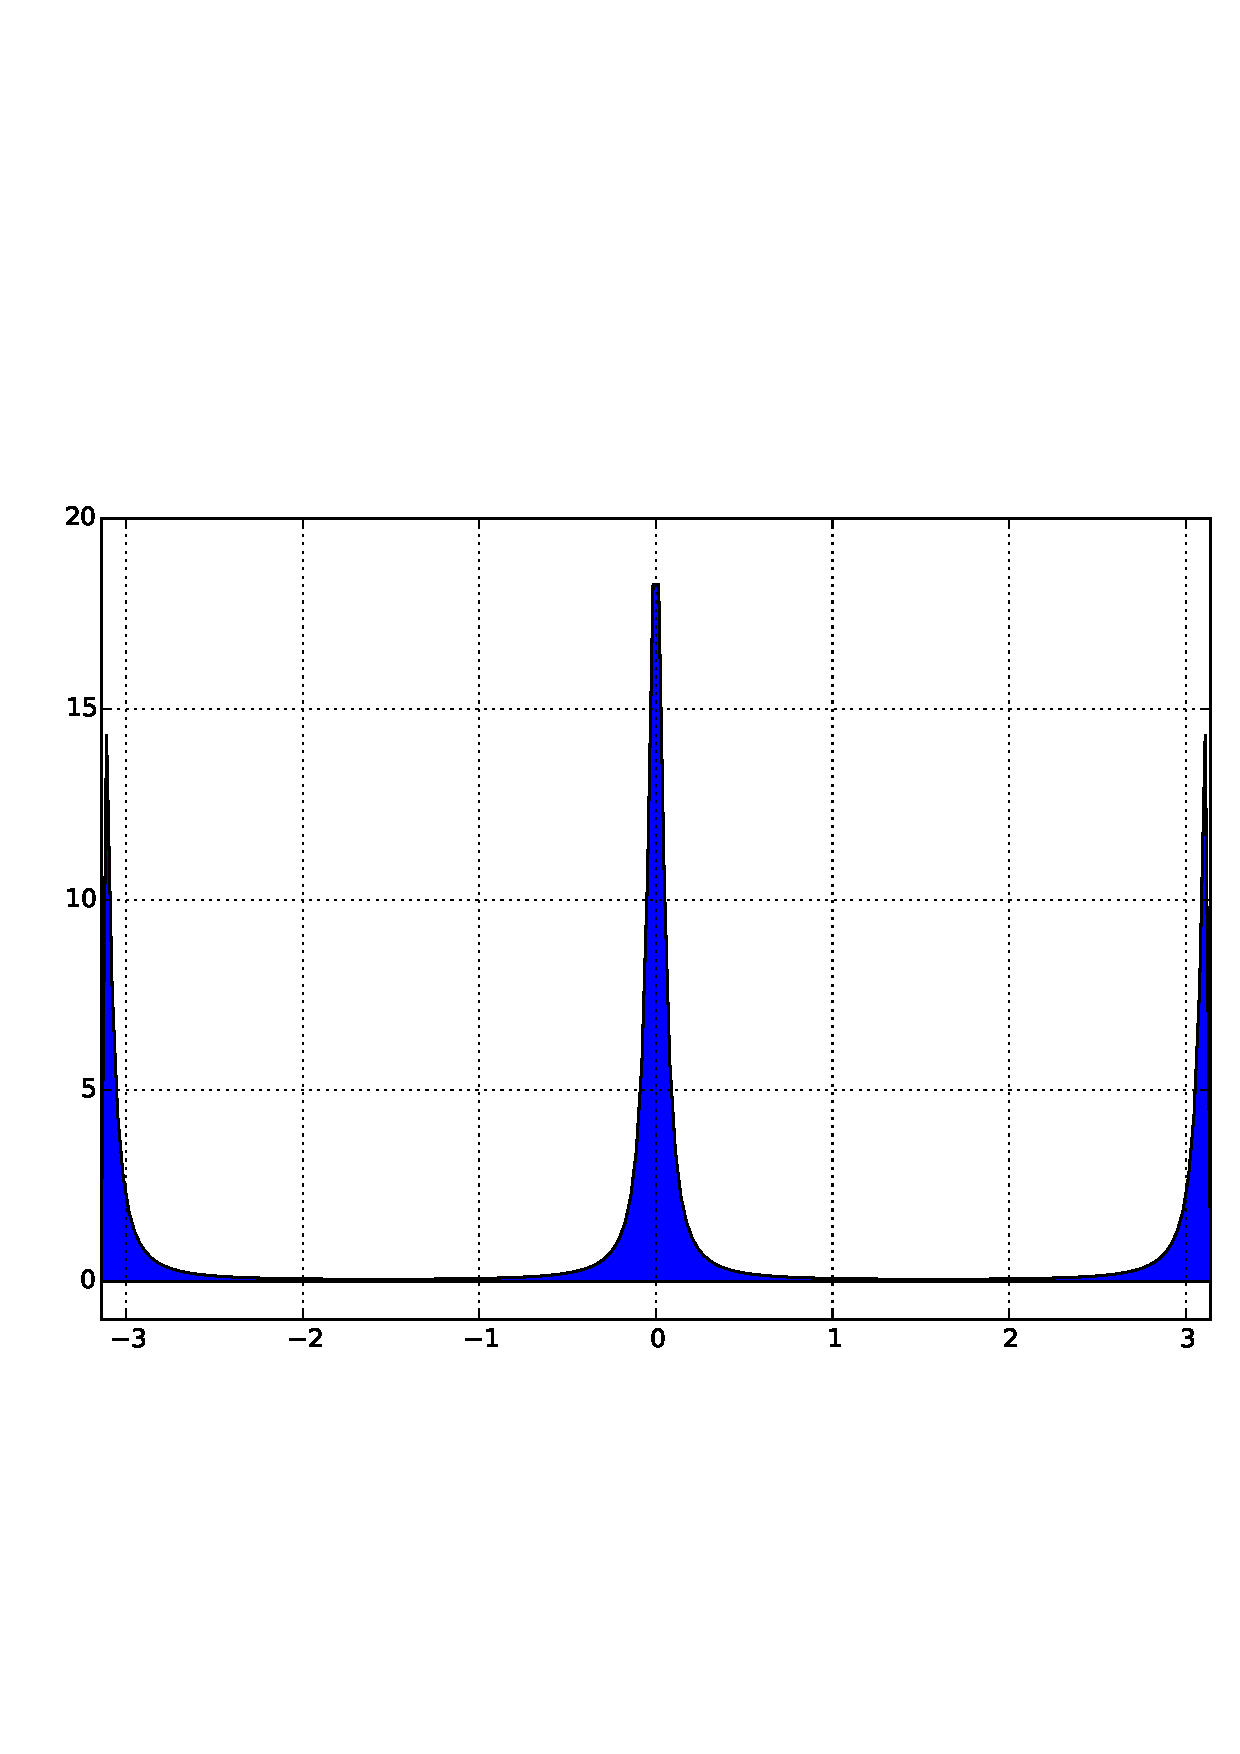
\includegraphics[width=\textwidth]{./images/exact_1D.pdf}
		\caption{Exact}
		\label{fig:exact}
	\end{subfigure}
	\begin{subfigure}{0.3\textwidth}
		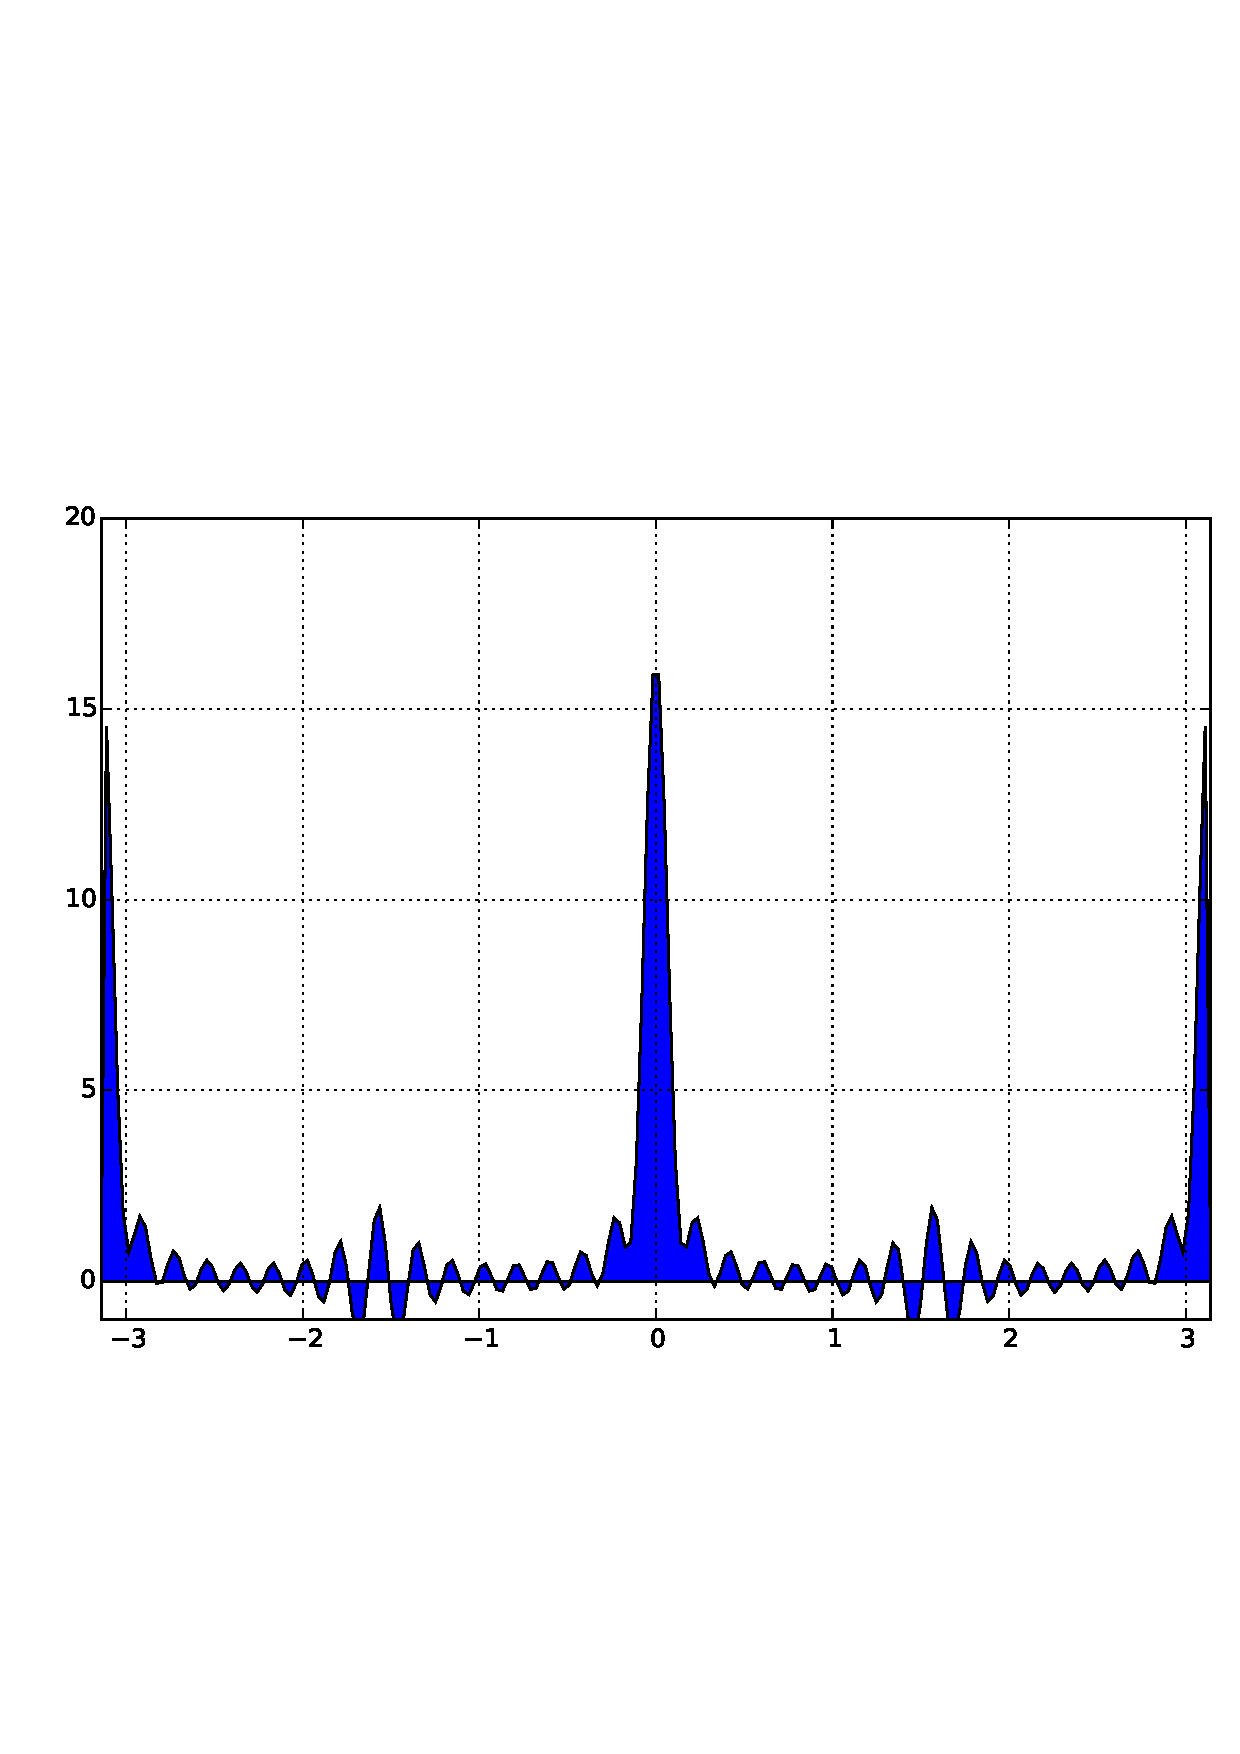
\includegraphics[width=\textwidth]{./images/standard_spectral_1D.pdf}
		\caption{Standard spectral}
		\label{fig:standard spectral}
	\end{subfigure}
	\begin{subfigure}{0.3\textwidth}
		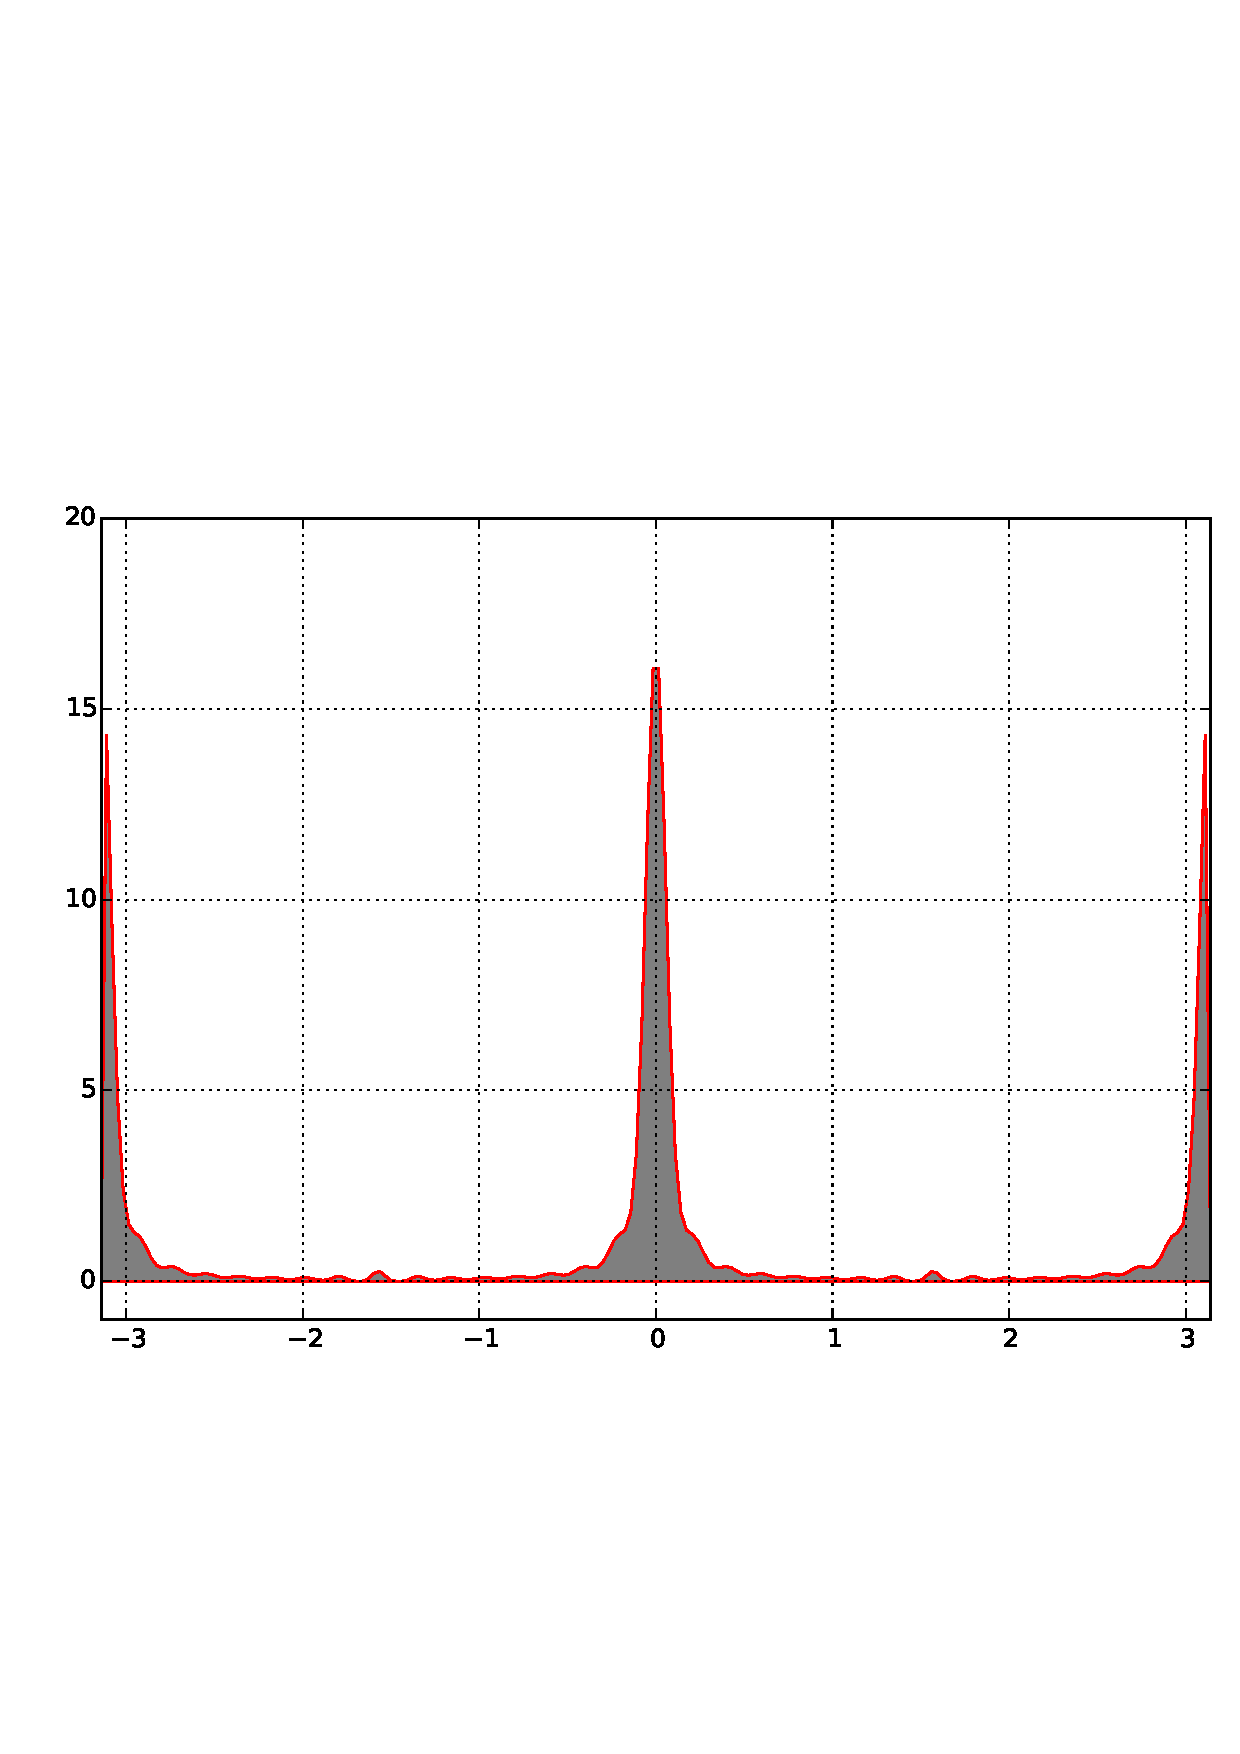
\includegraphics[width=\textwidth]{./images/gn_spectral_1D.pdf}
		\caption{GN spectral}
		\label{fig:gn spectral}
	\end{subfigure}
	\caption{A benchmark computation}
	\label{fig:S1}
\end{figure}

From these figures, it is tempting to suggest that GN discretization has greater qualitative accuracy than standard spectral discretization.
For one, standard spectral discretization exhibits negative mass, which is not physically achievable in the exact system.
Moreover, the $L^{1}$-norm is not conserved in standard spectral discretization.  However, by Theorem \ref{thm:norms} we know that
the $L^{1}$ norm is conserved in GN discretization.
A plot of the $L^{1}$-norm is given in figure \ref{fig:L1}

\begin{figure}
	\centering
	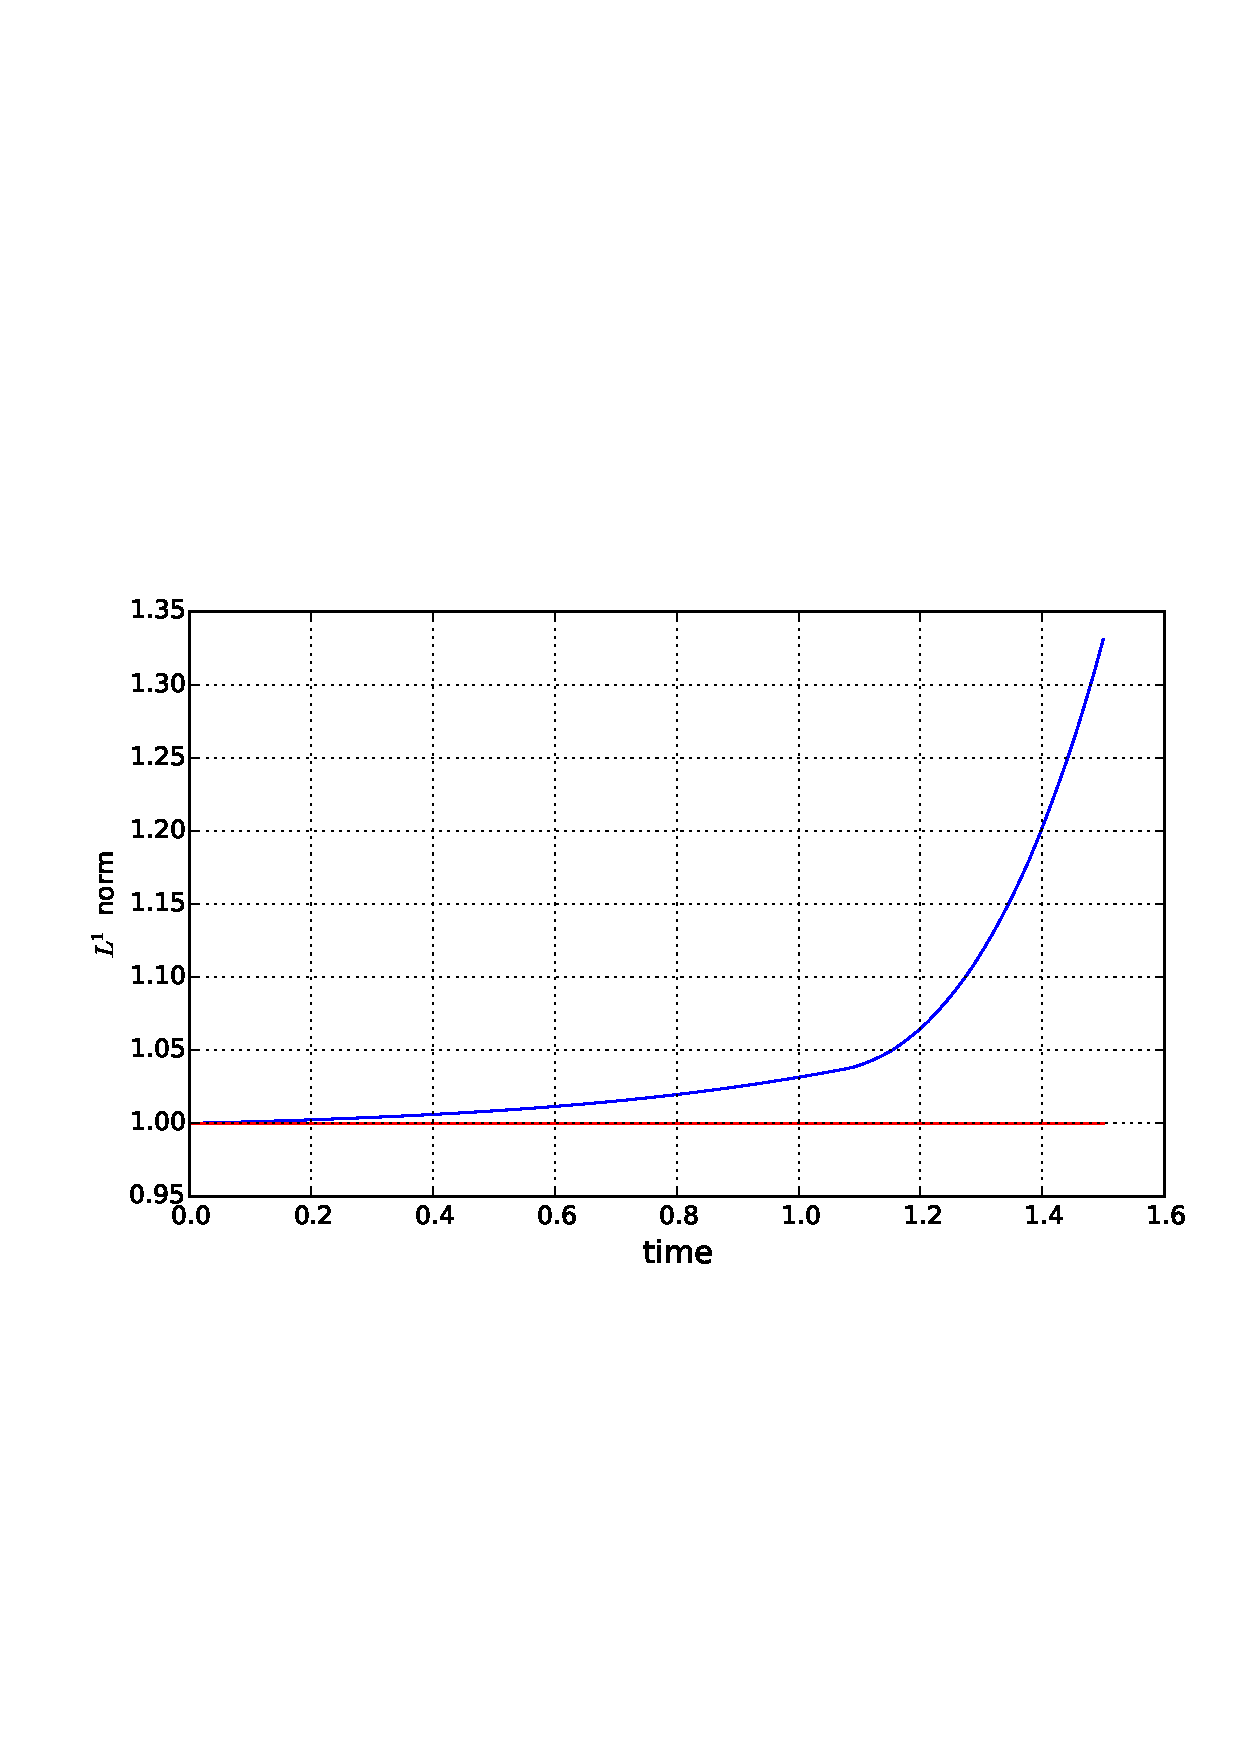
\includegraphics[width=0.8\textwidth]{./images/L1_plot.pdf}
	\caption{A plot of the $L^{1}$-norm vs time.
		The blue line denotes the $L^{1}$ norm under standard spectral discretization.
		The red line denotes the $L^{1}$ norm under GN discretization.
	}
	\label{fig:L1}
\end{figure}

We also know the evolution for an initial function, $f_{0}(x)$.
For example, if $f_{0}(x) = \sin(x)$ then the solution to \eqref{eq:function pde} under this vector-field is
\begin{align}
	f(x;t) = \frac{ e^{-2t} \sin(x) }{ \sqrt{ \cos^{2}(x) + e^{-4t} \sin^{2}(x) } }.
\end{align}

Unfortunately, algorithm 1 outputs $f$ as an operator on half-densities, and it is not clear how best to invert the hat-map.
However, we can obtain one estimate by applying $\hat{f}_{n}$ to the half-density $\sqrt{dx}$, and then divide the result by $\sqrt{dx}$.
The resulting function appears to approximate $f(x;t)$ well in the flat areas, and overshoot at the peaks.
In comparison, a standard spectral discretization seems to have large spurious oscillations in the center.
These estimates are plotted alongside the exact solution in figure \ref{fig:function}.
We should note that our means of converting $\hat{f}_{n}$ into a function is probably not the best choice of a left inverse to the hat-map.
Different choices yield different approximations to $f(x;t)$, some
of which get the peaks correct, but do poorly in the valleys.

We can see that the $L^{\infty}$-norm behaves well using GN discretization.
The $L^{\infty}$-norm is conserved to machine precision for GN discretization, while it will drift using standard discretization.

\begin{figure}
	\centering
	\begin{subfigure}{0.45\textwidth}
		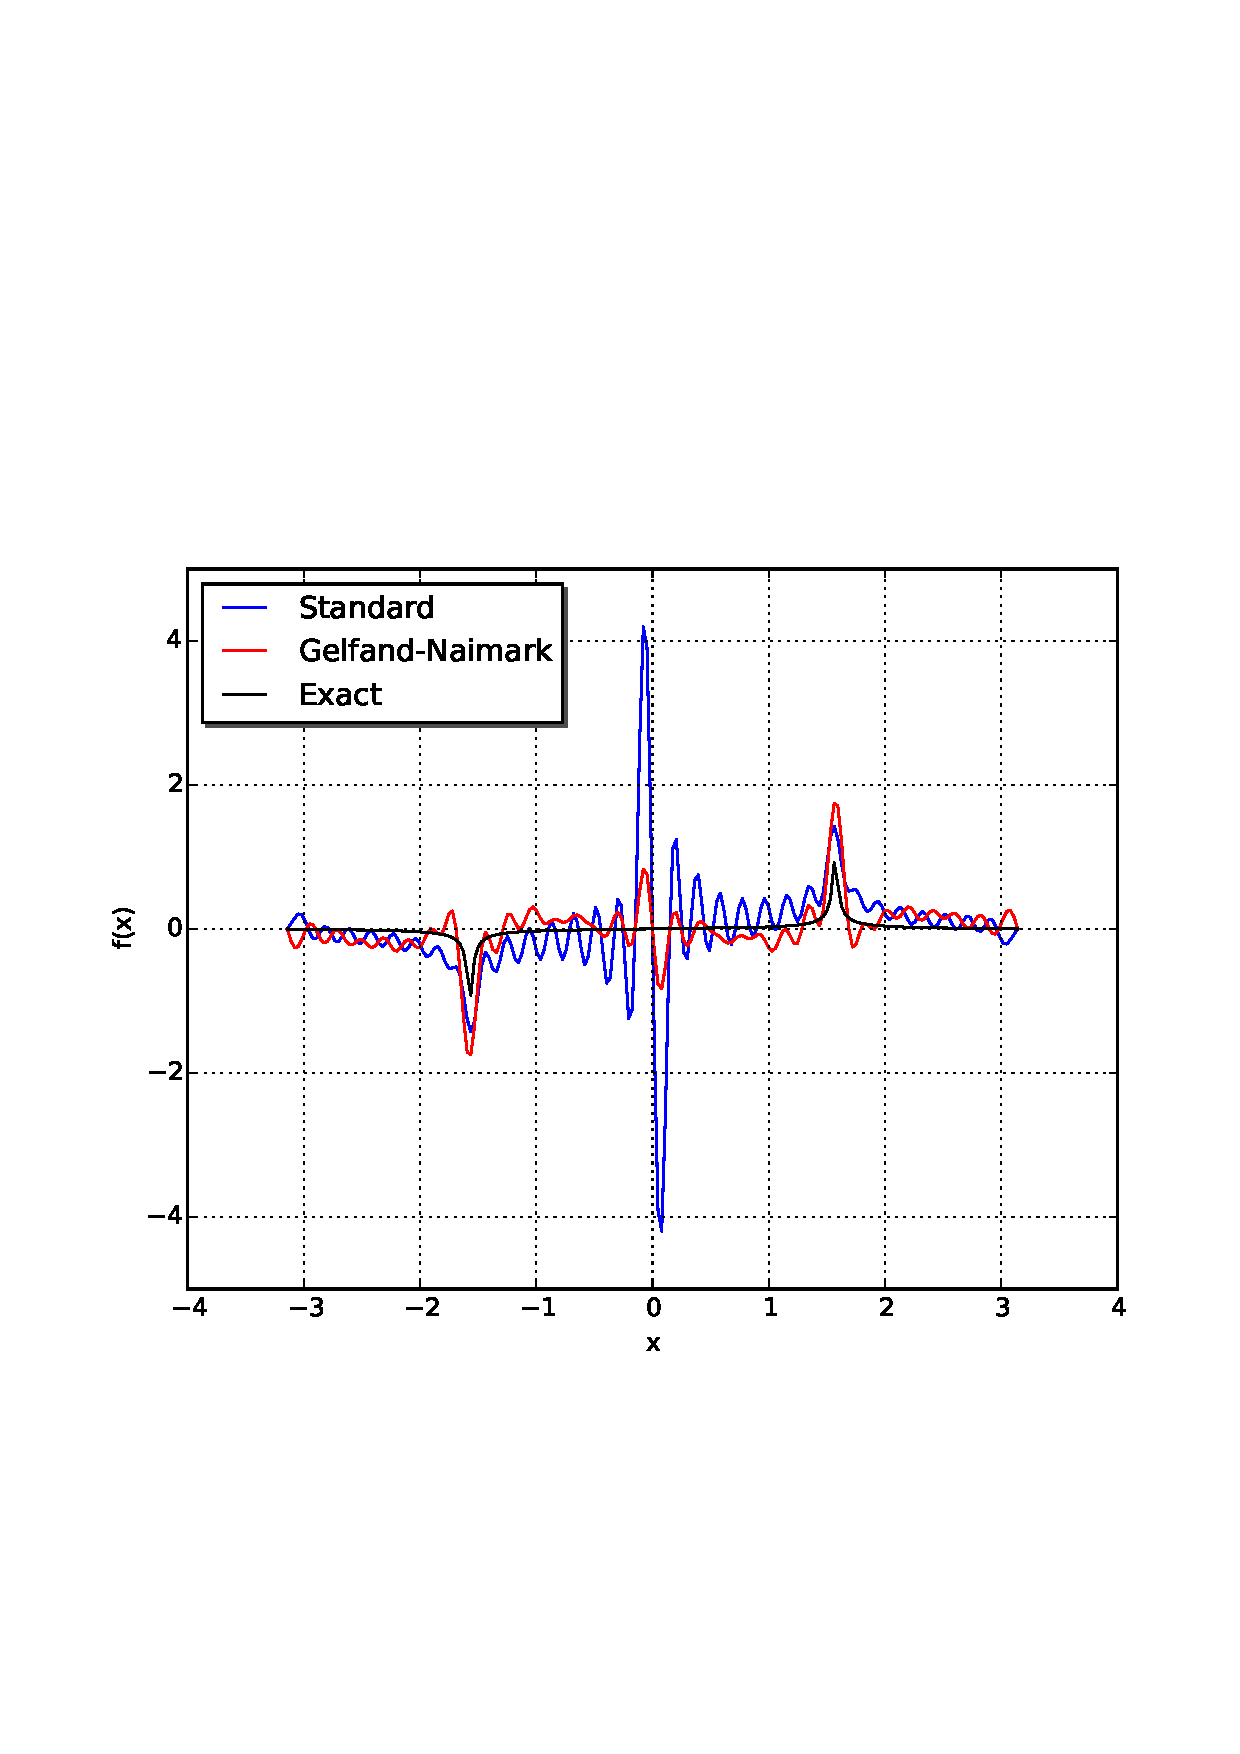
\includegraphics[width=\textwidth]{./images/function_comparison.pdf}
		\caption{Functions}
		\label{fig:function}
	\end{subfigure}
	\begin{subfigure}{0.45\textwidth}
		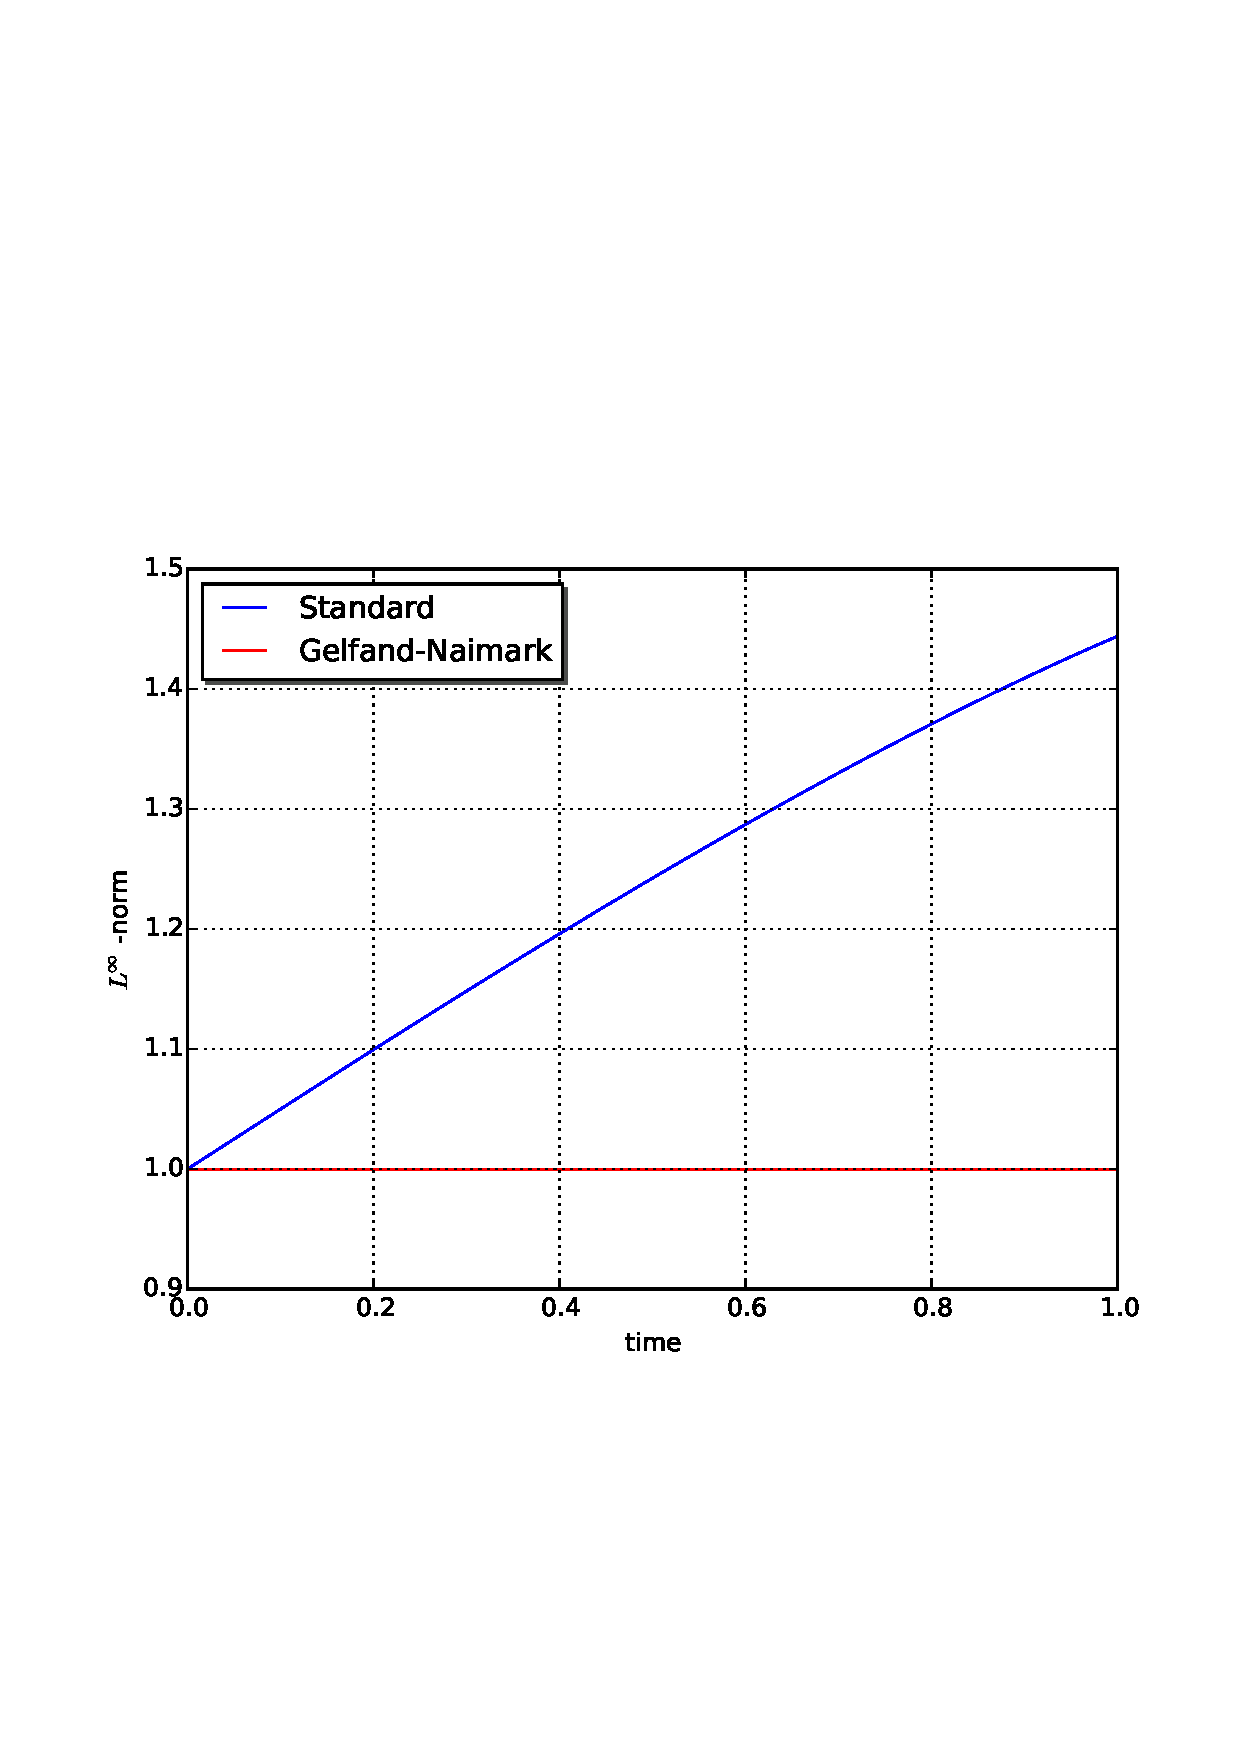
\includegraphics[width=\textwidth]{./images/L_inf_plot.pdf}
		\caption{$L^{\infty}$-norms}
		\label{fig:sup norm}
	\end{subfigure}
\end{figure}

\subsection{A system on the 2-torus}
Let us consider the system on $\mathbb{T}^{2}$ given by 
\begin{align}
	\dot{x} &= \cos(y) - D \sin(x) \\
	\dot{y} &= -\sin(x) - D \cos(y).
\end{align}
This can be seen as a dissipative Hamiltonian system with Hamiltonian $H(x,y) = \sin(y) - \cos(x)$ and dissipation $\vec{F} = D \cdot \nabla H$.
In Figure \ref{fig:2 torus} we depict the result of solving \eqref{eq:density pde} using three methods: GN spectral, Monte-Carlo, and a standard spectral discretization.
The top row depicts the result from applying algorithm 2 with the Fourier basis $\{ e^{2\pi i (k_{1}x +k_{2}y)} \mid -8 \leq k_{1},k_{2} \leq 8\}$.
This is a total of $289$ basis functions. 
The middle row depicts the results of a Monte-Carlo simulation with $10^{5}$ particles.
Finally, the bottom row depicts the results of a standard spectral scheme using the same basis as mentioned earlier.
The Monte-Carlo simulation can serve us as a benchmark.
We see that spurious oscillations will manifest using standard discretization, just as in the one-dimensional case.
Also as before, our GN discretization will conserve mass while the standard spectral scheme will dissipate and diffuse mass (by allowing for negative mass)

\begin{figure}
	\centering
	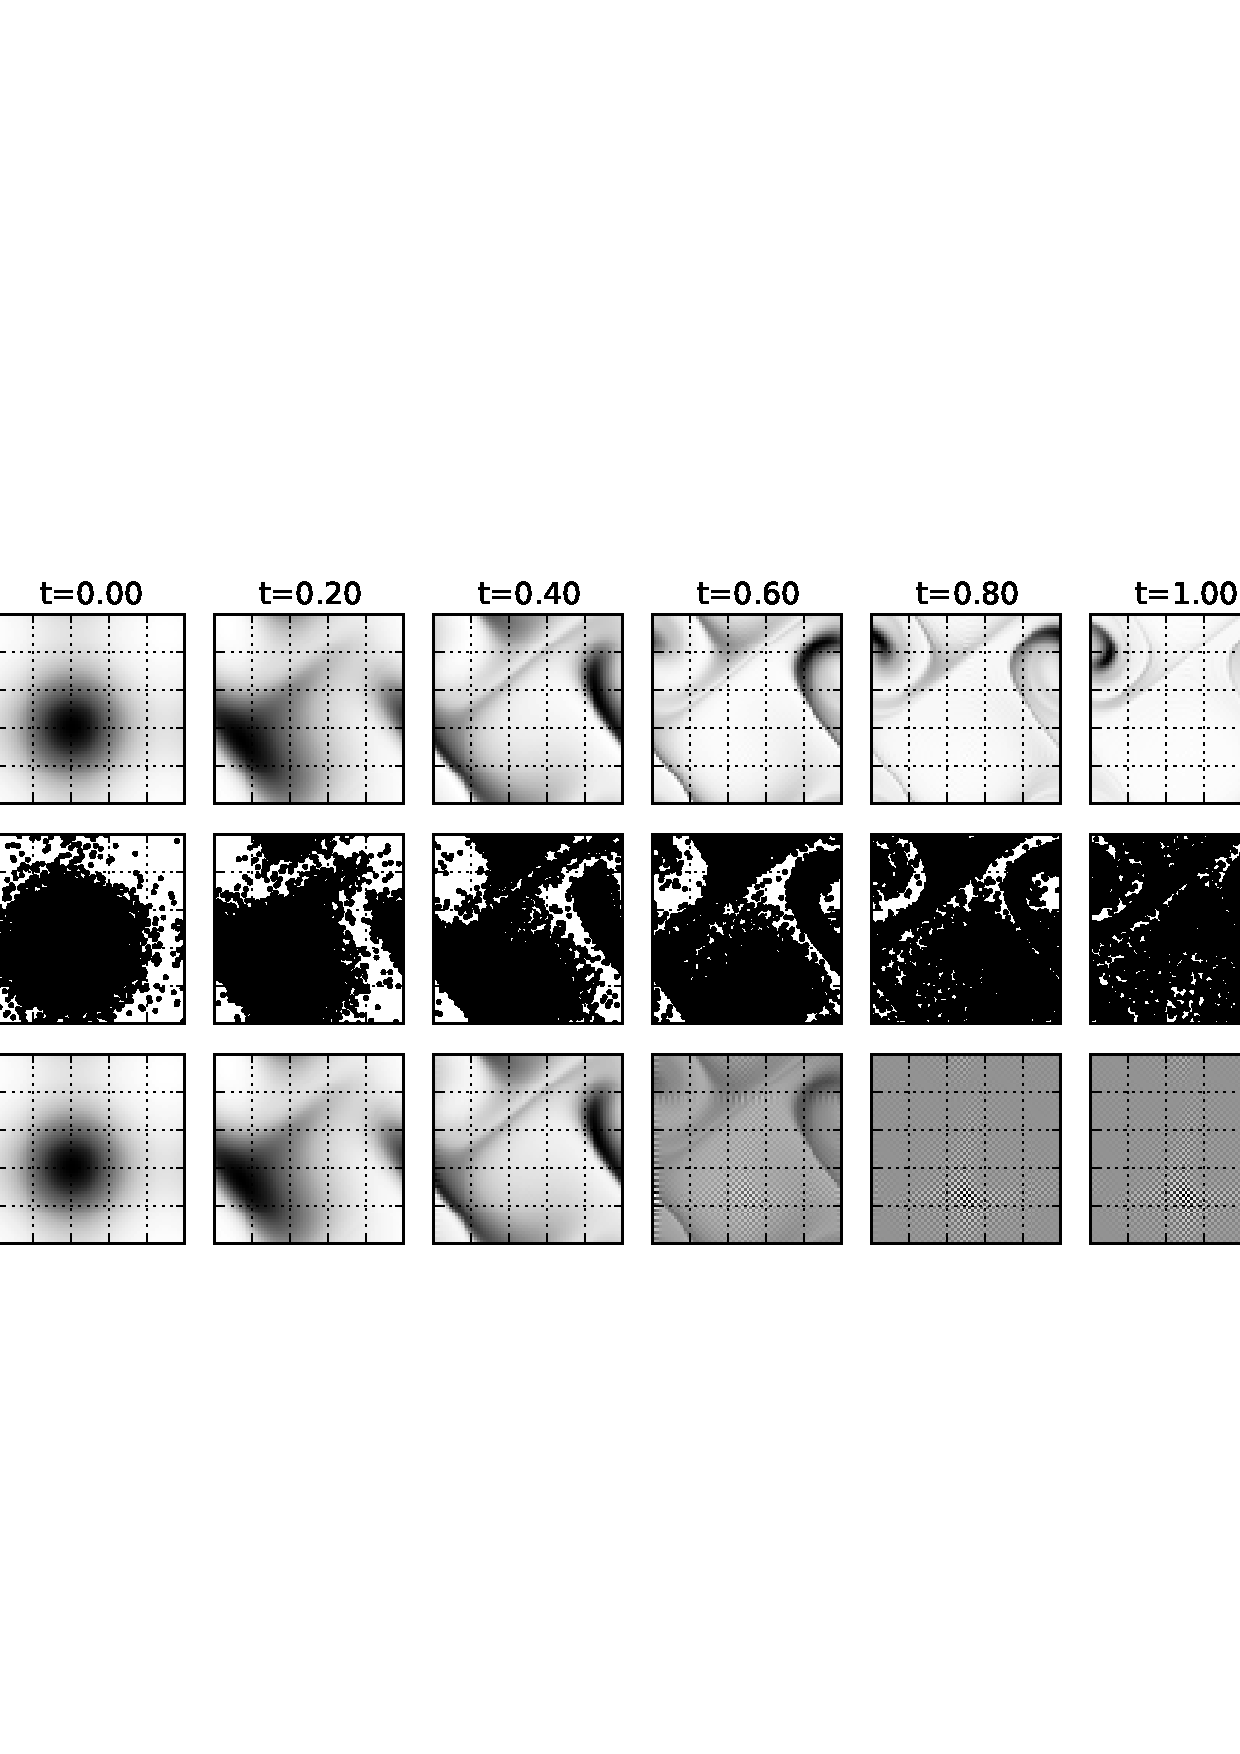
\includegraphics[width=0.8\textwidth]{./images/two_torus.png}
	\caption{Blah}
	\label{fig:2 torus}
\end{figure}


\subsection{Rigid body}
\todo[inline]{Do this last, if at all}

\subsection{ABC flow}
\todo[inline]{Only do densities, Plot location of mode,compare with Monte Carlo and standard spectral. Show slices, no fancy 3d shit.}

\section{Interpretations from $C^{*}$-algebras and quantum mechanics}

\todo[inline]{Things to mention: Gelfand transform, that \eqref{eq:half density pde} is a Shrodinger equation, reconstruction theorems.  That $\Diff(M)$ is the space of $*$-automorphisms.}

\section{Conclusion}

\subsection{Future work}

\todo[inline]{Boundary conditions, non-compact mfds}

\subsection{Acknowledgements}

\todo[inline]{Peter Michor, Stephen Marsland, Stefan Sommer}

\appendix

\section{Proof that $\pi$ is bracket preserving} \label{app:Lie}
Here we prove that $\pi$ is a Lie algebra morphism.

\section{A perturbed Gronwall's inequality}
\begin{lem} \label{lem:Gronwall}
If $\frac{du}{dt} \leq Ku + \epsilon$ then $u(t) \leq (\epsilon t + u(0) ) e^{Kt}$.
\end{lem}
\begin{proof}
	Let $w (t)= u (t) e^{-Kt}$.  Then for $t \geq 0$ we find
	\begin{align}
		\frac{dw}{dt} = \frac{du}{dt} e^{-Kt} - K w \leq (Ku+\epsilon) e^{-Kt} - Kw = \epsilon e^{-Kt} \leq \epsilon
	\end{align}
	Thus $w(t) \leq \epsilon t + w(0) = \epsilon t + u(0)$.
\end{proof}

\bibliographystyle{amsalpha}
\bibliography{hoj.bib}
\end{document}
